\documentclass[11pt,a4paper]{tesis}

\usepackage{graphicx}
\usepackage[utf8]{inputenc}
\usepackage[spanish]{babel}
\usepackage[left=3cm,right=3cm,bottom=3.5cm,top=3.5cm]{geometry}
\usepackage{amssymb}
\usepackage{float}
\usepackage{titlesec}
\usepackage{pdfpages}
\usepackage{fancyvrb}
\usepackage{xcolor}
\usepackage{amsthm}
\usepackage{amsmath}
\usepackage{cite}
\usepackage{mathtools}
\usepackage{hyperref}

\theoremstyle{definition}
\newtheorem{definition}{Definición}[section]
\titleformat*{\subsubsection}{\large\bfseries}
\newcommand*{\fvtextcolor}[2]{\textcolor[HTML]{#1}{#2}}
\DefineVerbatimEnvironment{Code}{Verbatim}{fontfamily=courier}

\begin{document}

\def\titulo{Licenciado }
\def\autor{Ivan Pasquini}
\def\tituloTesis{Localización y modelado simultáneos \mbox{mediante} generación y actualización \mbox{automática} de controladores discretos}
\def\runtitulo{Localización y modelado simultáneos mediante generación y actualización automática de controladores discretos}
\def\runtitle{Localización y modelado simultáneos mediante generación y actualización automática de controladores discretos}
\def\director{Nicolás Roque D'Ippolito}
\def\codirector{Leandro Ezequiel Nahabedian}
\def\lugar{Buenos Aires, 2016}
\newcommand{\HRule}{\rule{\linewidth}{0.2mm}}
%
\thispagestyle{empty}

\begin{center}\leavevmode

\vspace{-2cm}

\begin{tabular}{l}

\includegraphics[width=2.6cm]{logofcen.pdf}
\end{tabular}


{\large \sc Universidad de Buenos Aires

Facultad de Ciencias Exactas y Naturales

Departamento de Computaci\'on}

\vspace{6.0cm}

%\vspace{3.0cm}
%{
%\Large \color{red}
%\begin{tabular}{|p{2cm}cp{2cm}|}
%\hline
%& Pre-Final Version: \today &\\
%\hline
%\end{tabular}
%}
%\vspace{2.5cm}

{\huge\bf \tituloTesis}

\vspace{2cm}

{\large Tesis presentada para optar al t\'{\i}tulo de\\
\titulo en Ciencias de la Computaci\'on}

\vspace{2cm}

{\Large \autor}

{LU: 141/09}

\end{center}

\vfill

{\large

{Director: \director}

\vspace{.2cm}


\lugar
}

\newpage\thispagestyle{empty}


\frontmatter
\pagestyle{empty}
%\begin{center}
%\large \bf \runtitulo
%\end{center}
%\vspace{1cm}
\chapter*{\runtitulo}

\noindent
En el área de robótica, el problema de la exploración consiste en recorrer, mediante un vehículo autónomo,
una zona desconocida para obtener conocimiento sobre ella. La utilización de robots es muy importante para
la cartografía o búsqueda y rescate en lugares que son peligrosos o inaccesibles para las personas.\\
En el caso de la utilización de robots autónomos, se utiliza la técnica de localización y modelado simultáneos, 
para construir un mapa de la zona desconocida en la que se encuentra el robot, a la vez que estima su 
trayectoria al desplazarse dentro de la misma.

\vspace{\baselineskip}
El objetivo de esta tesis es resolver el problema de localización y modelado simultáneos utilizando como modelo 
matemático los MTS (Modal Transition System), que son nociones abstractas de los LTSs (Labelled Transition Systems).\\
Dado conjunto de objetivos y un conjunto de suposiciones de dominio, los MTSs nos permiten determinar, mediante la 
síntesis de controladores, si los objetivos son imposibles de realizar, si podemos garantizar su cumplimiento, o si 
las suposiciones de dominio son insuficientes para decidir sobre los objetivos.

\vspace{\baselineskip}
Para cumplir con el objetivo de la tesis, extenderemos la herramienta MTSA (Modal Transition System Analyser) para
dar soporte a la exploración, y presentaremos una estrategia, que bajo ciertas condiciones, nos permita ir agregando 
información a nuestras suposiciones de dominio, hasta poder decidir si es o no posible garantizar el cumplimiento de
los objetivos de la exploración.

\bigskip

\noindent\textbf{Palabras claves:} Exploración, Modelado, LTS, MTS, Síntesis de controladores.

\clearpage
\chapter*{Agradecimientos}

\noindent
A mi familia, sin su soporte incondicional no me hubiera sido posible llegar a este punto.\\ 
A mis amigos, quienes me acompañaron durante todos estos años de carrera.


\noindent A mi director de tesis y colaboradores, Leandro Nahabedian, Nicolás 
D'Ippolito 
y Natalia Rodriguez, por su guía, consejo y tiempo.

\noindent Al jurado, por haberse dedicado a la lectura y corrección de esta 
tesis.

\cleardoublepage
\hfill \textit{A mi familia}

\clearpage
\tableofcontents

\mainmatter
\pagestyle{headings}

\chapter{Introducción}

\section{Motivación}

En el área de robótica, el problema de la exploración consiste en recorrer, mediante un robot autónomo, una zona 
desconocida para obtener el conocimiento total de esta, o en caso de no poder reconocerla en su totalidad, maximizar 
el espacio explorado. 


La utilización de robots es muy importante para la cartografía o búsqueda y rescate en lugares que son peligrosos o 
inaccesibles para las personas. Hay muchos ejemplos de exploración con robots autónomos, como las sondas espaciales 
no tripuladas que exploran lugares antes de que lleguen los astronautas, o robots que ingresan en estructuras colapsadas 
para crear una reconstrucción del entorno y reconocer exactamente el lugar en el que se encuentran las víctimas.


Los robots autónomos necesitan un mapa para poder operar en un entorno particular. Por esta razón, se utiliza la técnica 
de localización y modelado simultáneos, para construir un mapa de una zona desconocida en la que se encuentra el robot, 
a la vez que estima su trayectoria al desplazarse dentro de la misma.


Existen trabajos previos que logran generar un mapa mediante exploración, trabajando sobre entornos estáticos. 
Se utilizan diversas técnicas para el aprendizaje sobre el entorno, como por ejemplo redes neuronales \cite{TP2}, 
grafos \cite{TP4} o múltiples robots \cite{TP5}. Algunos trabajos dejan abierta la pregunta sobre como explorar 
entornos dinámicos \cite{TP1} \cite{TP3}. También existen trabajos previos que contemplan cambios en el entorno \cite{TP6}.


En este trabajo estamos interesados en decidir si es posible alcanzar un 
objetivo (posición) en el mapa evitando lo maximo posible que el robot explore 
la totalidad del mapa. 
Dicho problema fue explorado 
en~\cite{melchior2007particle} ampliando el algoritmo tradicional que otorga 
un camino hacia el objetivo para que soporte incertidumbre del area a recorrer. 

\section{Resumen de la contribución}

Las contribuciones de esta tesis pueden verse desde un punto de vista teórico. 
Durante los últimos años, para resolver problemas de alcanzabilidad de un 
objetivo en una area, se han usado algoritmos basados en camino mínimo como 
Dijkstra, A*, entre otros. Sin embargo, este trabajo queda como evidencia de 
que nuevas estrategias pueden usarse. Decidimos utilizar algoritmos de síntesis 
de controladores para poder resolver el problema descrito.

Por otro lado, las técnicas existentes de síntesis de controladores nos 
permiten hallar una estrategia para el robot cuando el area a transitar es 
totalmente conocida. Para casos donde esta suposición del ambiente es muy 
fuerte, actualmente, no existe forma de obtener un plan adecuado. La forma 
natural de modelar un area parcialmente conocida es mediante el modelado de un 
MTS (Modal Transition System), formalismo matemático que introduciremos en la 
sección~\ref{sec:MTS}. 

Previo a nuestro trabajo, la síntesis de controladores para dichos ambientes 
genera una respuesta trivaluada: ``Sin importar cómo se resuelvan las 
incertidumbre del ambiente, SIEMPRE obtendremos un plan para llegar al 
objetivo'', ``Sin importar cómo se resuelvan las incertidumbres del ambiente, 
NUNCA obtendremos un plan para llegar al objetivo'' o ``depende de cómo se 
resuelvan las incertidumbres''. Como contribución, extenderemos esta respuesta 
para que, en los casos favorables, además de asegurarnos la existencia, nos de 
el plan para llegar al objetivo.

En resumen, lo que queremos es poder dar una respuesta certera a si es posible 
garantizar 
el cumplimiento del objetivo. 
Para lograrlo necesitamos explorar para adquirir nueva información en caso de 
que la información que poseemos no sea 
suficiente para dar una respuesta. Extenderemos la herramienta MTSA (Modal 
Transition System Analyser) para dar soporte 
a la exploración y presentaremos una estrategia que nos permita dar una 
respuesta certera sobre la posibilidad de 
cumplimiento del objetivo.


\section{Esquema de la tesis}

A continuación, en el capítulo 2, introduciremos la teoría sobre la cual se 
sustenta nuestra 
solución al problema. 
En este capítulo definiremos formalmente la matemática necesarias que 
posteriormente vamos a utilizar. Luego, en el capítulo 3, introduciremos, 
formalmente, el problema a resolver. Presentaremos un algoritmo que lo resuelve 
y una posible estrategia de exploración que garantice encontrar una respuesta a 
este problema. El capítulo 4 muestra resultados de nuestra técnica.
Para ello, mostraremos como se comporta nuestro algoritmo y nuestra estrategia 
frente a una serie de problemas que servirán para mostrar las características 
de nuestra implementación. Despues en el capítulo 5, daremos conclusiones de 
este trabajo. Analizaremos el algoritmo y la estrategia, y plantearemos que 
trabajos a futuro podrían hacerse a partir de esta tesis. 
Finalmente, en el capítulo 6 y a modo de apendice, adjuntamos el manual de 
usuario para exploración en la herramienta MTSA basado en un ejemplo.

\chapter{Fundamentos teóricos}

\section{El mundo y la maquina}
El modelo del mundo y la máquina de Michael Jackson \cite{MundoMaquina} es una abstracción que permite formular rigurosamente algunas nociones
fundamentales de la ingeniería de requerimientos. En este modelo, los fenómenos son hechos, situaciones o eventos cuya
existencia puede observarse, la maquina es una porción del sistema a desarrollar o modificar y el mundo es una porción de
la realidad afectada por la máquina. El mundo y la máquina interactúan en la interfaz de la máquina. Un problema del mundo 
describe una parte del mundo real que nosotros queremos mejorar construyendo la solución como una máquina.

\vspace{\baselineskip} 
En este modelo, los requerimientos R son declaraciones prescriptivas (propiedades deseadas que pueden cumplirse o no) sobre 
el mundo expresadas en términos de fenómenos sobre la interfaz entre la máquina que queremos construir y el mundo en el cual 
viven los problemas que queremos resolver. Los requerimientos deben ser forzados por la maquina independientemente de cómo 
se comporte el mundo. Los problemas del mundo son capturados como declaraciones prescriptivas expresadas en término de 
fenómenos del mundo llamados objetivos G, y declaraciones descriptivas (propiedades sobre el sistema que se mantienen 
independientes a cómo se comporta el sistema) sobre lo que nosotros asumimos que es verdad en el mundo, suposiciones 
de dominio D. Las suposiciones de dominio podrían no mantenerse y deben ser satisfechas por el mundo. 

\vspace{\baselineskip}
La tarea clave de la ingeniera de requerimientos es comprender y documentar los objetivos y las características del entorno.
Teniendo estos modelos se pueden formular un conjunto de requerimientos para la máquina de forma que en conjunto con el
entorno satisfagan los objetivos. Más formalmente R, D $\vDash$ G.
Esto puede ser formulado como un problema de síntesis \cite{Sintesis}. Dados un conjunto de suposiciones del dominio y un conjunto de
objetivos del sistema, construir  automáticamente un modelo operacional de la maquina tal que compuesto con el modelo del
entorno, los objetivos sean alcanzados.

\vspace{\baselineskip}
Diremos que un evento es controlable si es controlable por la máquina. Una evento es monitoreable o no controlable si es
controlable por el mundo. 
Para cumplir los objetivos, el modelo operacional restringe la ocurrencia de eventos controlables basándose en la observación
de los eventos que ya ocurrieron.
Este problema se conoce como el problema de síntesis de controladores y está siendo estudiado exhaustivamente en varios
aspectos de la ingeniería de los requerimientos.

\section{Labelled Transition Systems}
Los Labelled Transition Systems \cite{LTS} (LTSs) son ampliamente utilizados para modelar y analizar el comportamiento de sistemas
concurrentes y distribuidos. Son un sistema de transición de estados en el cual las transiciones son etiquetadas con
acciones. El conjunto de acciones de un LTS se conoce como alfabeto comunicacional y constituye las interacciones que
el sistema modelado puede tener con el entorno.

\begin{definition}{(Labelled Transition System)}
Sea $Estados$ el conjunto universal de estados y $Acciones$ el conjunto universal de etiquetas de acciones. Un Labelled
Transition System es una tupla $E = (S_{E}, A_{E}, \Delta_{E}, s_{0}^{E})$ en donde $S_{E} \subseteq Estados$ es un conjunto
finito de estados, $A_{E} \subseteq Acciones$ es un alfabeto finito, $\Delta_{E} \subseteq (S_{E} \times A_{E} \times S_{E})$ es una
relación de transición y $s_{0}^{E} \in S_{E}$ es el estado inicial.
\end{definition}

Dado $(s, l, s$’$) \subseteq \Delta_{E}$ decimos que $l$ está habilitada desde $s$ en $E$. Decimos que un LTS es
determinístico si desde un estado, al realizar una acción, hay solo un estado posible al que llegamos.

\section{Composición en paralelo}

Sean $M$ y $E$ dos LTSs. La composición en paralelo $\parallel$ es un operador simétrico que crea un nuevo LTS $M \parallel E$, 
tal que sus estados son el producto cartesiano de los estados de $M$ y $E$, sus acciones la unión de las acciones de $M$ y $E$, 
y su función de transición sincroniza el movimiento de las dos máquinas en las acciones compartidas, mientras que se 
mueven independientemente en sus acciones propias.

\begin{definition}{(Composición en paralelo)}
Sean $M = (S_{M}, A_{M}, \Delta_{M}, s_{0}^{M})$ y\\
$N = (S_{N}, A_{N}, \Delta_{N}, s_{0}^{N})$ dos LTSs. Composición en paralelo $\parallel$ es un operador simétrico tal que 
$M \parallel N$ es el LTS $P = (S_{M} \times S_{N}, A_{M} \cup A_{N}, \Delta_{P}, (s_{0}^{M}, s_{0}^{N}))$, donde $\Delta_{P}$ es
la menor relación que satisface las siguientes reglas:

\vspace{\baselineskip}
$\dfrac{(s, l, s') \in \Delta_{M}}{((s, t), l, (s', t)) \in \Delta_{P}}$ con $l \in A_{M} \setminus A_{N}$

\vspace{\baselineskip}
$\dfrac{(t, l, t') \in \Delta_{N}}{((s, t), l, (s, t')) \in \Delta_{P}}$ con $l \in A_{N} \setminus A_{M}$

\vspace{\baselineskip}
$\dfrac{(s, l, s') \in \Delta_{M}, t, l, t') \in \Delta_{N}}{((s, t), l, (s', t')) \in \Delta_{P}}$ con $l \in A_{M} \cap A_{N}$
\end{definition}

\section{LTS Legal}
Dados dos LTSs $N$ y $M$, y $A_{N_{u}} \subseteq A_{N}$, decimos que $M$ es un Legal LTS para $N$ respecto a $A_{N_{u}}$ si por cada
estado en $E\parallel$$M$, realizar una acción perteneciente a $A_{N_{u}}$ es igual a realizar la acción en $N$.
Intuitivamente, en la composición una acción es deshabilitada si y solo si también es deshabilitada en el LTS original.
En otras palabras, $M$ no restringe a $N$ respecto a $A_{N_{u}}$.

\begin{definition}{(LTS Legal)}
Sean $M = (S_{M}, A_{M}, \Delta_{M}, s_{0}^{M})$ y $N = (S_{N}, A_{N}, \Delta_{N}, s_{0}^{N})$ dos LTSs y sea $A_{N_{u}} \in A_{N}$ un estado.
Decimos que $M$ es un LTS legal para $N$ respecto a $A_{N_{u}}$, si para todo ($s_{n}, s_{m}) \in E \parallel M$ pasa que 
$\Delta_{E \parallel M}((s_{n}, s_{m})) \cap A_{N_{u}} = \Delta_{N}(s_{N}) \cap A_{N_{u}}$.
\end{definition}

\section{Traza}
Una traza es una secuencia de acciones ejecutadas en un LTS. Una traza puede ser finita o infinita.

\begin{definition}{(Traza)}
Sea $E = (S_{E}, A_{E}, \Delta_{E}, s_{0}^{E})$ un LTS. Una secuencia $\pi = l_{0}, l_{1}, ...$ es una traza en $E$ si existe una
secuencia $s_{0}, l_{0}, s_{1}, l_{1}, ...$ en donde para todo $i \geq 0$ vale $(s_{i}, l_{i}, s_{i + 1}) \in \Delta_{E}$.
\end{definition}

\section{Bisimulación}

La bisimulación es una relación de equivalencia entre LTSs.

\begin{definition}{(Bisimulación)}
Sea $L$ el universo de todos los LTSs. Una relación binaria $R \subseteq L \times L$ es una bisimulación sí y solo sí cuando 
$(P, Q) \in R$ entonces para cada acción $a \in A_{P} \cup A_{Q}$:

\begin{itemize}

\item
$(P \xrightarrow{a} P') \Rightarrow (\exists Q' \cdot Q \xrightarrow{a} Q' \land (P', Q') \in R)$

\item
$(Q \xrightarrow{a} Q') \Rightarrow (\exists P' \cdot P \xrightarrow{a} P' \land (P', Q') \in R)$

\end{itemize}

\end{definition}


\section{Bisimilaridad}

La equivalencia entre LTSs se define mediante la noción de bisimilaridad.

\begin{definition}{(Bisimilaridad)}
Sea $L$ el universo de todos los LTSs. Dos LTSs $P, Q \in L$ son bisimilares sí y solo sí existe una bisimulación $R$ tal que $(P, Q) \in R$.

\end{definition}

\section{Modal Transition System}
Los Modal Transition System \cite{MTS} (MTS), son nociones abstractas de los LTSs. Extienden a los LTSs ya que las transiciones 
que los MTSs poseen, pueden denotar eventos requeridos o bien posibles. Debido a esta particularidad de los MTSs, es 
que podemos modelar mediante este formalismo información parcial del mundo.

\vspace{\baselineskip}
La definición es la misma que para LTSs, pero la función de transición se divide en dos para separar las acciones
requeridas de las posibles. Las posibles incluyen a las requeridas.

\begin{definition}{(Modal Transition System)}
Sea $Estados$ el conjunto universal de estados y $Acciones$ el conjunto universal de etiquetas de acciones. Un Modal
Transition System es una tupla $M = (S_{M}, A_{M}, \Delta_{M}^{r}, \Delta_{M}^{p}, s_{0}^{M})$ en donde $S_{M} \subseteq Estados$
es un conjunto finito de estados, $A_{M} \subseteq Acciones$ es un alfabeto finito, 
$\Delta_{M}^{r} \subseteq \Delta_{M}^{p} \subseteq (S_{M} \times A_{M} \times S_{M})$ son las relaciones de transición requeridas
y posibles respectivamente, y $s_{0}^{M} \in S_{M}$ es el estado inicial.
\end{definition}

\section{Refinamiento}
Hay una relación de refinamiento entre los MTSs y los LTSs. Un LTS se puede ver como un MTS en donde la función de
transición de las acciones posibles es igual que la función de transición de las acciones requeridas. Los LTSs que
refinan un MTS son descripciones completas del comportamiento del sistema y se llaman implementaciones.

\begin{definition}{(Refinamiento)}
Sean $M = (S_{M}, A, \Delta_{M}^{r}, \Delta_{M}^{p}, s_{0}^{M})$ y\\
$N = (S_{N}, A, \Delta_{N}^{r}, \Delta_{N}^{p}, s_{0}^{N})$ dos MTSs. La relación $H \subseteq S_{M} \times S_{N}$ es un refinamiento
entre $M$ y $N$ si para todo $l \in A$, $(s_{M}, s_{N}) \in H$ se cumple:

\begin{itemize}

\item
Si $(s_{M}, l, s_{M}') \in \Delta_{M}^{r}$ entonces existe $s_{N}'$ tal que $(s_{N}, l, s_{N}') \in \Delta_{N}^{r}$ y $(s_{M}', s_{N}') \in H$.

\item
Si $(s_{N}, l, s_{N}') \in \Delta_{N}^{p}$ entonces existe $s_{M}'$ tal que $(s_{M}, l, s_{M}') \in \Delta_{M}^{p}$ y $(s_{M}', s_{N}') \in H$.

\end{itemize}

Decimos que $N$ refina a $M$ si existe una relación de refinamiento $H$ entre $M$ y $N$ tal que $(s_{0}^{M}, s_{0}^{N}) \in H$.

\end{definition}

\section{Implementación}

\begin{definition}{(Implementación)}
Un LTS $L$ es una implementación de un MTS $M$ si y solo si $L$ refina a $M$.
\end{definition}

Una implementación es deadlock free si todos sus estados tienen transiciones salientes.
Un MTS es determinístico si ninguna de sus acciones conduce desde un estado a más de un estado.

\section{Fluent}

Los fluents nos permiten especificar propiedades basadas en estados, en modelos basados en eventos.

\begin{definition}{(Fluent)}
Sea $Acciones$ el conjunto universal de etiquetas de acciones.
Un fluent es es una tupla $Fl = \langle I_{fl}, T_{fl}, Init_{fl} \rangle$ en donde $I_{fl} \subseteq Acciones$ son las acciones
que inicializan, $T_{fl} \subseteq Acciones$ las que terminan y $Init_{fl} \in \{true, false\}$ indica el estado inicial.
\end{definition}

\section{Fluent Linear Temporal Logic}
Fluent Linear Temporal Logic \cite{FLTL} (FLTL) es una lógica temporal lineal que nos permite razonar sobre fluents.

\begin{definition}{(Fluent Linear Temporal Logic)}
Sea $Acciones$ el conjunto universal de etiquetas de acciones y $\Pi$ el conjunto de posibles trazas infinitas sobre $Acciones$.
Una formula FLTL se define inductivamente usando los conectores Booleanos standard y los operadores temporales \textbf{X} (Next) y
\textbf{U} (strong until) de la siguiente forma:\\
$\varphi ::= Fl | \neg\varphi | \varphi \lor \psi | \textbf{X}\varphi | \varphi\textbf{U}\psi$ donde $Fl \in Fluents$.
\end{definition}

Dada una traza, por cada posición en la traza podemos decidir si el fluent está activo o no.

\begin{definition}{(Satisfacción)}
Sea $Acciones$ el conjunto universal de etiquetas de acciones, $Fluents$ el conjunto de todos los posibles fluents sobre $Acciones$,
y $\Pi$ el conjunto de posibles trazas infinitas sobre $Acciones$. La traza $\pi \in \Pi$ satisface el el fluent $Fl \in Fluents$ en
la posición $i$ si y solo si vale alguna de las siguientes condiciones:

\begin{itemize}

\item
$Init_{Fl} \land (\forall j \in \mathbb{N} \cdot 0 \leq j \leq i \rightarrow l_{j} \notin T_{Fl})$

\item
$\exists j \in \mathbb{N} \cdot (j \leq i \land l_{j} \in I_{Fl}) \land (\forall k \in \mathbb{N} \cdot j \leq k \leq i \rightarrow 	l_{k} \notin T_{Fl})$

\end{itemize}

Dada una traza infinita $\pi$, la satisfacción de una formula $\varphi$ en la posición $i$, denotada $\pi, i\vDash \varphi$ se define de la siguiente forma:

\begin{itemize}
\item
$\pi, i\vDash Fl \triangleq \pi, i\vDash Fl$
\item
$\pi, i\vDash \neg\varphi \triangleq \neg(\pi, i\vDash \varphi)$
\item
$\pi, i\vDash \varphi \lor \psi \triangleq (\pi, i\vDash \varphi) \lor (\pi, i\vDash \psi)$
\item
$\pi, i\vDash \textbf{X}\varphi \triangleq \pi, 1\vDash \varphi$
\item
$\pi, i\vDash \varphi\textbf{U}\psi \triangleq \exists j \geq i \cdot \pi, j \vDash \psi \land \forall i \leq k < j \cdot \pi, k \vDash \varphi$
\end{itemize}

Decimos que $\varphi$ se sostiene en $\pi$ si $\pi, 0\vDash \varphi$. Una formula $\varphi \in FLTL$ se sostiene en un LTS $E$ si se sostiene en cada traza
infinita producida por $E$.

\end{definition}


\section{Generalised Reactivity (1)}

Dada una secuencia infinita de estados, una formula GR(1) \cite{SRD} denota cuales han ocurrido infinitamente. 
Más formalmente, $\phi = (A, B)$ en donde $A$ y $B$ son conjuntos de subconjuntos de estados en donde o bien alguno de los
subconjuntos de $A$ no contiene ningún estado que se visita infinitamente, o bien todos los subconjuntos de $B$ contienen 
al menos un estado que se visita infinitamente.

\begin{definition}{(Generalised Reactivity (1))}
Sea $Estados$ el conjunto universal de estados. Dada una secuancia infinita de estados $p$, sean $inf(p)$ los estados que
ocurren infinitamente en $p$. Sea $\phi_{1}, ..., \phi_{n}$ y $\varUpsilon_{1}, ..., \varUpsilon_{m}$ subconjuntos de $Estados$. Sea\\
$gr((\phi_{1}, ..., \phi_{n}), (\varUpsilon_{1}, ..., \varUpsilon_{m}))$ el conjunto de infinitas secuencias $p$ tales que
o bien para algun $i$ vale $inf(p)\cap\phi_{i} = \varnothing$ o para todo $j$ vale $inf(p)\cap\varUpsilon_{j} \neq \varnothing$.
\end{definition}

\section{Síntesis de controladores}

La síntesis de controladores se encarga de producir automáticamente una máquina que restringe la ocurrencia de eventos
controlables basándose en la observación de los eventos que ya ocurrieron. Cuando esta máquina es desplegada en un ambiente
adecuado garantiza la satisfacción de un conjunto de objetivos dado. La satisfacción de estos objetivos depende de la
satisfacción de las asunciones sobre el entorno.

\subsection{LTS control problem}

Podemos describir la síntesis de controladores de la siguiente forma. Dados un LTS que describe el comportamiento
del entorno, un conjunto de acciones controlables, un conjunto de fórmulas FLTL que representan las suposiciones
del dominio y un conjunto de fórmulas FLTL que representan los objetivos del sistema, el problema de control de
LTS \cite{LTSControl} es encontrar un LTS que solo restrinja la ocurrencia de acciones controlables y garantice que la composición
en paralelo entre el ambiente y el LTS es deadlock free y que si las suposiciones de dominio se satisfacen, entonces
los objetivos del sistema también son satisfechos. Intuitivamente, al resolver un problema de síntesis, buscamos evitar alcanzar
estados para los cuales no se puedan satisfacer los objetivos. Estos estados no deseables los vamos a llamar estados perdedores.
Las zonas inseguras son conjuntos de estados perdedores.

\begin{definition}{(LTS control)}
Dado un modelo del domino en forma de un LTS determinístico $E = (S_{E}, A_{E}, \Delta_{E}, s_{0}^{E})$, un conjunto de
acciones controlables $A_{c} \subseteq A_{E}$ y una formula FLTL $\varphi$, la solución al LTS control problem
$\varepsilon = \langle E, \varphi, A_{c} \rangle$ es un LTS $M = (S_{M}, A_{M}, \Delta_{M}, s_{0}^{M})$ tal que
$A_{M} = A_{E}$, y por cada estado en $S_{M}$ todas las acciones en $A_{M} \setminus A_{c}$ estás habilitadas, $E \parallel M$
es deadlock free, y toda traza $\pi$ en $E \parallel M$ garantiza $\pi \vDash \varphi$
\end{definition}

El LTS Control Problem es decidible en tiempo exponencial y en caso de ser decidible, se encuentra la solución con la
misma complejidad. Para esto es necesario que el modelo sea determinístico.

\subsection{MTS	control problem}

El problema de la síntesis de controladores para MTSs \cite{MTSControl} consiste en ver si todas, alguna o ninguna de sus implementaciones
pueden ser controladas por un controlador LTS. Al responder esta pregunta, también estamos respondiendo la pregunta de
si el problema es realizable, ya que si la respuesta es ninguno el problema no es realizable. Para decidir este problema,
primero se intenta encontrar un controlador para la implementación del MTS que tiene todas las acciones posibles controlables.
Si se lo encuentra, se tiene un controlador para todas las posibles implementaciones. Se hace lo mismo con el que tiene la
mínima cantidad de acciones controlables y así se obtiene la respuesta.

\begin{definition}{(MTS control)}
Dado un modelo del domino en forma de un MTS $M = (S_{M}, A, \Delta_{M}^{r}, \Delta_{M}^{p}, s_{0}^{M})$, un conjunto de
acciones controlables $A_{c} \subseteq A_{M}$ y una formula FLTL $\varphi$, la solución al MTS control problem
$\varepsilon = \langle M, \varphi, A_{c} \rangle$ es responder:

\begin{itemize}

\item
\textbf{All} si para todo LTS $I$ que sea implementación de $M$, el LTS control problem $\langle I, \varphi, A_{c} \rangle$ es realizable.

\item
\textbf{None} si para ningún LTS $I$ que sea implementación de $M$, el LTS control problem $\langle I, \varphi, A_{c} \rangle$ es realizable.

\item
\textbf{Some} en otro caso.

\end{itemize}

\end{definition}

\section{Finite State Process}
El Finite State Process (FSP) \cite{FSP} es un lenguaje de especificación semántica bien definida en términos de LTSs que nos permite describirlos en
forma concisa. El lenguaje puede extenderse para poder describir MTSs.
\chapter{Síntesis de controladores en entornos parcialmente conocidos}

Nuestro problema consiste en dado una posición inicial del sistema y un punto 
fisico objetivo dentro de una area/habitación, es requerido transladarnos al 
punto deseado. La particularidad de el problema a resolver es la falta de 
información que tenemos sobre el area donde transitar. Diremos entonces que 
buscaremos soluciones al problema de navegación de robots cuando el entorno es 
parcialmente conocido.
Tenemos un objetivo, pero no sabemos lo suficiente sobre el entorno como para 
decidir si es 
posible satisfacerlo. Debemos obtener el conocimiento necesario sobre el 
entorno para poder decidir sobre el objetivo. 
Por otro lado, el entorno puede ser tanto estático como dinámico. Será dinámico 
en caso de que mientras el robot intenta santisfacer su objetivo, existan 
componentes externos cuyas acciones modifican la configuración inicial del area 
a explorar.
Para lograrlo, vamos a utilizar los sensores del robot, los cuales nos aportan 
información, y una estrategia que 
utilice el conocimiento adquirido para obtener conocimiento nuevo.

Cuando comenzamos la exploración, la información que tenemos sobre el mundo es 
parcial. Los MTSs nos permiten codificar
la incertidumbre, ya que podemos distinguir la información que poseemos como 
transiciones requeridas y la información
que podemos adquirir mediante exploración como transiciones posibles. El mundo 
real, el cual estamos explorando, puede 
representarse como un LTS (Labelled Transition System) que refina nuestro MTS 
inicial.

Además del LTS que representa al mundo real, otros LTSs pueden refinar al MTS 
que representa nuestro conocimiento. Estos
LTSs representan a todas las posibles formas que puede llegar a tener el mundo 
real a partir del conocimiento que poseemos
actualmente. En cada uno de estos LTSs, las acciones posibles o bien van a ser 
acciones requeridas, o bien no van a formar
parte del LTS, y en caso de que sean acciones requeridas, puede variar la 
cantidad de veces que puede ejecutarse dicha acción.
Por estas razones, la cantidad de LTSs que refinan a nuestro MTS puede llegar a 
ser infinita. Cada uno de estos LTSs está
decidiendo sobre la incertidumbre del MTS que representa nuestro conocimiento 
actual.

Cuando exploramos, lo hacemos para poder realizar un objetivo. Mediante la 
síntesis de controladores, podemos intentar 
generar automáticamente una máquina, tal que al componerla en paralelo con el 
MTS que representa nuestro conocimiento 
del mundo, garantice el cumplimiento del objetivo.

Si para cada uno de los LTSs que refinan a nuestro MTS, el objetivo es 
alcanzable, sabemos que podemos garantizar el
cumplimiento del objetivo, ya que el mundo puede representarse como un LTS que 
refina nuestro modelo. Cuando no es posible
sintetizar un controlador que pueda garantizar que los objetivos se alcancen 
para ninguno de los LTSs que refinan a nuestro
modelo, podemos afirmar que el objetivo no es realizable en el mundo real. Pero 
si para algunos de estos LTSs existe un
controlador, y para otros no, no podemos afirmar nada sobre nuestro objetivo.

\section{Problema}

Una posible solución al problema de la síntesis de controladores en entornos 
parcialmente conocidos es un LTS $x$ (ver sección~\ref{sec:LTS}) tal que 
$M$ $\parallel$ $x$ $\models$ $G$, en donde $M$ es el MTS (ver 
sección~\ref{sec:MTS}) que modela el entorno y $G$ es un fórmula en FLTL (ver 
sección~\ref{sec:FLTL}) que describe cual es el sector objetivo. 

El estado del arte en cuanto a síntesis de controladores sobre Modal Transition 
Systems, nos otorga una respuesta trivaluada como mostramos previamente en la 
sección~\ref{sec:MTS_control}. Sin embargo, actualmente no existe forma de 
obtener un LTS solución ($x$). Si bien una de nuestras contribuciones es 
generar automáticamente el LTS $x$, la complejidad de producir dicho output 
depende de la configuración inicial de nuestros inputs. 
Por lo tanto podemos detallar tres casos al momento inicial de la ejecución:

\begin{itemize}

\item
\textit{Es posible sintetizar el LTS $x$ para cualquier implementación de $M$.} 
En otras 
palabras, sabemos que para toda incertidumbre que se encuentre en el area, sin 
importar qué encontremos al explorar esa zona, tenemos una estrategia que nos 
lleva al punto objetivo.

\item
\textit{No es posible sintetizar el LTS $x$ para ninguna implementación de 
$M$.} Esto es que sin importar como se resuelvan las incertidumbres, el sistema 
nunca va a poder alcanzar el objetivo.

\item
\textit{Algunas implementaciones de $M$ ofrecen buenas garantías para 
satisfacer el 
objetivo pero otras no. }
Por lo tanto, no sabemos si es posible sintetizar un controlador para la implementación de $M$ que representa al mundo real, el cual no conocemos.

\end{itemize}

En los dos primeros escenarios tenemos una respuesta a nuestro problema. De estar en el tercer escenario, queremos poder sintetizar 
el controlador en caso de ser posible, o tener garantías de que es imposible sintetizar dicho controlador. Para lograr nuestro objetivo 
debemos agregar información a M, para poder reducir su cantidad de posibles implementaciones, y que, de esta forma, su síntesis caiga 
en uno de los dos primeros escenarios.

La exploración nos permite adquirir conocimiento, ya que al observar mediante los sensores del robot lugares del entorno en los cuales 
no habíamos estado, podemos despejar la incertidumbre en nuestro modelo del entorno, representado por M. Vamos a realizar la exploración 
mediante un algoritmo, el cual se basa en ciclos de adquisición de conocimiento. Si nuestra información sobre el entorno es insuficiente, 
movemos al robot para que pueda aprender algo nuevo. Repetimos el ciclo hasta poder dar una respuesta.

Más formalmente podemos definir el problema síntesis de controladores en entornos parcialmente conocidos de la siguiente manera:

\begin{definition}{(Síntesis de controladores en entornos parcialmente conocidos)}
Sea $G$ una fórmula en FLTL que representa los requerimientos del sistema y $M$ es un MTS que representa las suposiciones del dominio conocidas en el momento inicial. Resolver el problema de síntesis de controladores en entornos parcialmente conocidos es decidir si existe un LTS $x$ tal que $M' \| x \models G$ donde $M' \prec M$ que representa el conocimiento inicial del entorno más todo el conocimiento adquirido por la exploración.
\end{definition}

\section{Algoritmo}

\begin{figure}[H]
  \centering
    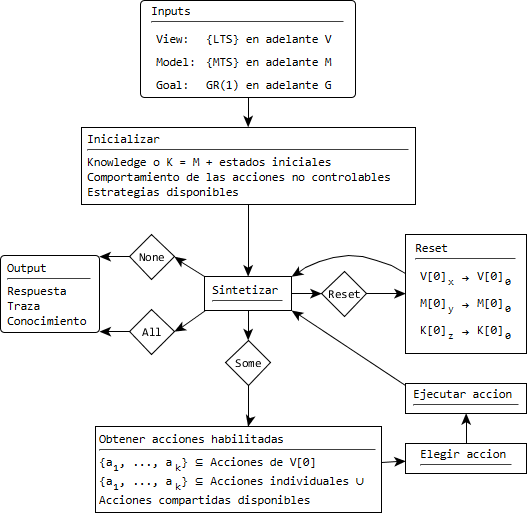
\includegraphics[scale=0.8]{Imagenes/Algoritmo/Algoritmo.png}
  \caption{Algoritmo de exploración.}
  \label{fig:Algoritmo}
\end{figure}

\begin{algorithm}
\begin{algorithmic}
\REQUIRE \{LTS\} View, \{MTS\} Model, GR(1) Goal
\ENSURE All si se puede satisfacer Goal en el Knowledge actual y None en caso contrario
\STATE Knowledge := Model $\cup$ estados iniciales
\STATE Respuesta := Sintetizar(Knowledge, Goal)
\WHILE {Respuesta == Some $||$ Respuesta == Reset}
\IF{Respuesta == Some}
\STATE Acciones habilitadas := \{a$_{1}$, ..., a$_{k}$\} tal que \{a$_{1}$, ..., a$_{k}$\} $\subseteq$ Acciones individuales(Knowledge[0]) $\cup$ Acciones compartidas disponibles(Knowledge[0])
\STATE Acción := Elegir(Knowledge, Acciones habilitadas)
\STATE Ejecutar(View, Model, Knowledge, Acciones controlables, Acción)
\ELSE
\STATE Reiniciar estados iniciales(View, Model, Knowledge)
\ENDIF
\STATE Respuesta := Sintetizar(Knowledge, Goal)
\ENDWHILE
\RETURN Respuesta
\end{algorithmic}
\caption{Algoritmo de exploración}
\end{algorithm}

\section{Inputs}

Para resolver el problema necesitamos poder observar al entorno a medida que nos movemos, saber con que información inicial 
contamos y tener un objetivo que cumplir.

\subsection{View}
\textbf{View} es una lista de LTSs. Representa el mundo sobre el cual se mueve el robot. 
El primer LTS de la lista representa el mapa del entorno, el cual regula como se mueve el robot por el mundo. Indica que acciones 
puede realizar en cada posición, y a que lugar lo llevan dichas acciones. 
Los otros LTSs representan el comportamiento de los agentes externos que interactúan con el entorno. Pueden bloquear y habilitar 
acciones en una determinada posición. El robot no tiene influencia sobre ellos. 
El robot solamente puede observar el estado actual del \textbf{View} mediante sus sensores. Sobre el mapa, solamente puede saber en qué posición 
está y que acciones puede ejecutar en dicha posición. Sobre los agentes externos, solamente puede observar su estado actual.

\subsection{Model}
\textbf{Model} es una lista de MTSs. Representa nuestro conocimiento inicial sobre el mundo. Por cada LTS en \textbf{View} hay un correspondiente MTS 
en \textbf{Model}. 
La única restricción para los MTSs de \textbf{Model}, es que puedan refinarse en sus correspondientes LTSs de \textbf{View}. Por lo tanto, como mínimo, 
cada MTS debe contar con un estado, y por cada acción en su correspondiente LTS, debe haber una acción posible en el MTS.

\subsection{Goal}
\textbf{Goal} es el objetivo del robot. Exploramos para poder decidir si es posible garantizar el cumplimiento de \textbf{Goal}. Está expresado con una 
fórmula GR\big(1\big).

\section{Inicialización}

\textbf{Knowledge} es una lista de MTSs que representa el conocimiento que vamos adquiriendo en cada iteración del algoritmo. En cada iteración, los MTSs 
de \textbf{Knowledge} son un refinamiento de los MTSs de la iteración anterior. Cada MTS de \textbf{Knowledge} se compone de dos grupos de estados: Los 
que están en \textit{La nube} y los que representan el conocimiento.


\textit{La nube} representa la incertidumbre. Es una copia del MTS de \textbf{Model}. Sus estados y acciones se mantienen inmutables en todas las 
iteraciones de \textbf{Knowledge}. 
El resto de los estados representan el conocimiento adquirido hasta el momento. Su cantidad de estados irá creciendo a medida que el robot adquiera información. 
En cada estado, las acciones que nunca fueron ejecutadas irán a un estado de 
\textit{La nube}, mientras que las que ya fueron ejecutadas, irán a un estado 
del conocimiento.


En la implementación del algoritmo en la herramienta MTSA, hay dos cuestiones importantes de inicialización. 
Por un lado, el comportamiento de las acciones no controlables de los agentes externos. Actualmente existen dos patrones de comportamiento. 
Por defecto, los agentes externos elegirán una acción al azar. El otro patrón de comportamiento consiste en que se comporten de forma cíclica ejecutando 
las acciones que nosotros pasamos como input. En el futuro podrá extenderse la herramienta con más patrones de comportamiento. 
La otra cuestión es la estrategia utilizada por el robot. En esta tesis presentamos una única estrategia que resuelve el problema, pero en el futuro puede 
extenderse la herramienta con estrategias diferentes.

\section{Síntesis}

\begin{figure}[H]
  \centering
    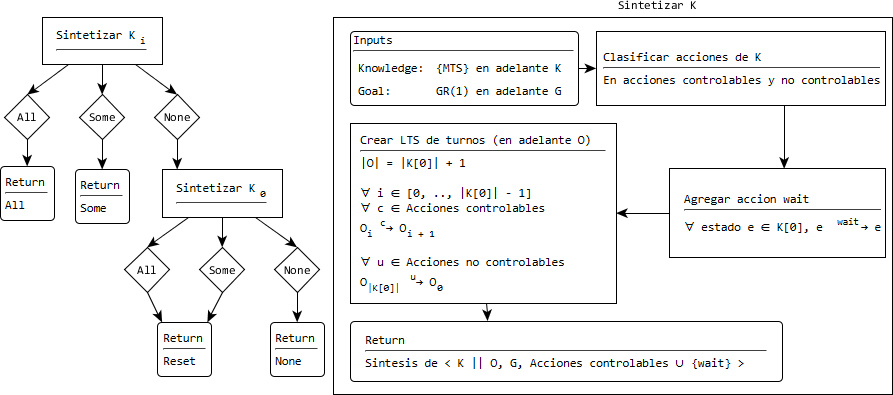
\includegraphics[width=1.0\textwidth]{Imagenes/Algoritmo/Algoritmo_sintetizar.png}
  \caption{Algoritmo de síntesis.}
  \label{fig:Algoritmo_sintetizar}
\end{figure}

\begin{algorithm}
\begin{algorithmic}
\REQUIRE \{MTS\} Knowledge, GR(1) Goal
\ENSURE Devuelve la respuesta al problema de control sobre Knowledge y Goal, o Reset si la respuesta es Some al volver la posición inicial de Knowledge al inicio
\STATE Knowledge en posición actual := Cambiar estado inicial a actual(Knowledge)
\STATE Respuesta := Problema de control(Knowledge en posición actual, Goal)
\IF{Respuesta == None}
\STATE Respuesta := Problema de control(Knowledge, Goal)
\IF{Respuesta == None}
\RETURN None
\ELSE
\RETURN Reset
\ENDIF
\ELSE
\RETURN Respuesta
\ENDIF
\end{algorithmic}
\caption{Algoritmo general de síntesis}
\end{algorithm}

\begin{algorithm}
\begin{algorithmic}
\REQUIRE \{MTS\} Knowledge, GR(1) Goal
\ENSURE La respuesta decide la realizabilidad de Goal sobre las implementaciónes de Knowledge
\STATE Acciones controlables := Obtener acciones controlables(Knowledge)
\STATE Acciones no controlables := Obtener acciones no controlables(Knowledge)
\FOR{Estado $\in$ Estados(Knowledge[0])}
	\STATE Agregar acción(Knowledge[0], WAIT, Estado, Estado)
\ENDFOR
\STATE LTS de turnos := Crear LTS de turnos(Knowledge, Acciones controlables, Acciones no controlables)
\STATE Respuesta := Síntesis(Knowledge $||$ LTS de turnos, Goal, Acciones controlables $\cup$ \{wait\})
\RETURN Respuesta
\end{algorithmic}
\caption{Algoritmo del problema de control sobre MTSs}
\end{algorithm}

\newpage

\subsection{Detalle}

Al principio de cada iteración, lo primero que hacemos es intentar dar una respuesta a la pregunta sobre si podemos garantizar el cumplimiento del objetivo. 
En otras palabras, queremos ver si podemos sintetizar un controlador que garantice el cumplimiento de \textbf{Goal}.

La síntesis la haremos sobre un MTS basado en \textbf{Knowledge}, pero con algunas modificaciones necesarias para modelar correctamente el problema. 
Primero cambiamos el estado inicial del primer MTS de \textbf{Knowledge}, el que representa el mapa, para que su estado inicial sea el estado en el que está 
situado actualmente el robot. Esto es para que el controlador garantice el objetivo desde nuestra posición actual.

Luego, al primer MTS de \textbf{Knowledge} (el mapa), le agregaremos en cada estado la acción controlable wait, que irá al mismo estado. 
Esto es para representar la posibilidad de que el robot espere en su posición actual un cambio en los agentes externos.

Por último, creamos un LTS de turnos que permita al robot moverse a cualquier estado antes de que los agentes externos realicen cambios. Esto es para evitar que los 
agentes externos esperen que el robot esté lejos para realizar una acción que beneficie al robot. El LTS de turnos permitirá que el robot se mueva una cantidad 
de veces igual a la cantidad de estados del primer MTS del \textbf{Knowledge} (el mapa) antes de que los agentes externos se muevan.

De esta forma, con la posibilidad de moverse y esperar en cualquier estado conocido, puede estar en el estado necesario para beneficiarse de las acciones de 
los agentes externos. Sintetizaremos el controlador para \textbf{Goal} sobre la composición en paralelo de los MTSs de \textbf{Knowledge}, incluyendo el MTS al 
cual le agregamos las acciones wait, con el LTS de turnos.

Si el resultado de la síntesis es que puede generarse un controlador para cualquier LTS que sea un refinamiento del MTS que armamos, significa que el robot 
puede cumplir el objetivo sin importar como sean las zonas inexploradas del entorno. El algoritmo termina, dando como resultado la garantía del cumplimiento 
de \textbf{Goal}.

En caso de que no pueda generarse un controlador mara ningún LTS que sea un refinamiento del MTS que armamos, hay que volver a realizar la síntesis, pero sin 
realizar el cambio del estado inicial. Si nuevamente no puede generarse un controlador, significa que es imposible cumplir \textbf{Goal}, sin importar como sean 
las zonas inexploradas del entorno, y el algoritmo termina confirmando la imposibilidad de cumplimiento de \textbf{Goal}. En caso contrario, significa que 
llegamos a un punto sin retorno, pero todavía hay zonas inexploradas que pueden ser alcanzadas desde el inicio, en las cuales podríamos o no cumplir el objetivo. 

En caso de que nuestro robot tenga la capacidad de volver al inicio, o utilizar otro robot desde la zona inicial, podemos seguir explorando cambiando los 
estados iniciales de los primeros componentes de \textbf{View}, \textbf{Model} y \textbf{Knowledge} (los que representan al mapa) al estado inicial del comienzo 
de la exploración. Al hacer esto contamos con la información recolectada hasta el momento, la cual puede utilizar la estrategia para no volver a caer en el 
punto sin retorno.

Por último, si la síntesis puede generar un controlador para algunas de las implementaciones del MTS que armamos, pero para otras no, significa que no tenemos 
suficiente información sobre el entorno como para decidir sobre el objetivo, y necesitamos seguir explorando para refinar el \textbf{Knowledge}.

\section{Estrategia}

En caso de que sea necesario seguir explorando, necesitamos que la estrategia decida la próxima acción a ejecutar. El algoritmo está preparado para que, 
al utilizar múltiples estrategias, detecte si alguna entra en un ciclo infinito y la reemplace por otra.

\begin{figure}[H]
  \centering
    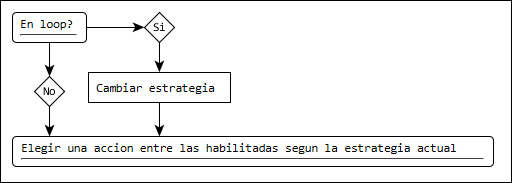
\includegraphics[scale=0.75]{Imagenes/Algoritmo/Algoritmo_elegir_1.png}
  \caption{Elección de estrategia}
  \label{fig:Algoritmo_elegir_1}
\end{figure}

\begin{algorithm}
\begin{algorithmic}
\REQUIRE \{MTS\} Knowledge, {Accion} Acciones habilitadas
\ENSURE Cambia la estrategia actual si entro en un ciclo
\IF{en un ciclo()}
\STATE Cambiar estrategia()
\ENDIF
\STATE Elegir(Knowledge, Acciones habilitadas)
\end{algorithmic}
\caption{Algoritmo de elección de estrategia}
\end{algorithm}


\subsection{Optimista}

Estamos por elegir una acción. Hacemos esto porque el intento de síntesis para generar un controlador que garantice \textbf{Goal} nos dio como resultado que 
existe un controlador para algunos refinamientos pero no para otros. En particular existe un controlador para el refinamiento más optimista, llamado 
controlador optimista. La estrategia Optimista aprovecha este hecho, ya que por construcción, el controlador optimista evitará las zonas inseguras. Lo que 
hace la estrategia es elegir de entre las acciones posibles, una acción que esté en el estado inicial del controlador optimista. En cambio, la estrategia 
Optimista - Nueva acción lo utiliza para filtrar de entre las acciones posibles, cuáles son las acciones seguras, y así elegir mediante la estrategia Nueva acción 
una acción entre las seguras.

\subsection{Nueva acción}

La estrategia Nueva acción tiene como objetivo ejecutar acciones nuevas, o en otras palabras, que no hayan sido ejecutadas anteriormente en su estado asociado. 
Si siempre ejecutamos acciones nuevas, siempre adquiriremos conocimiento nuevo, y como el entorno a explorar es finito, terminaremos por reconocerlo completamente 
de seguir esta estrategia.


La estrategia se divide en varias etapas. Lo primero que debemos hacer es saber sí, entre las acciones disponibles, existe alguna que no haya sido ejecutada 
anteriormente desde el estado actual. Si existe, la elegiremos, porque es una acción nueva.


Si el estado actual es un estado completamente explorado, o en otras palabras, ya ejecutamos anteriormente todas las acciones disponibles desde este estado, debemos 
llegar a un estado no completamente explorado. Para hacerlo, buscamos si hay algún estado que cumpla las condiciones deseadas al que podamos volver. Esto 
significa que exista un estado con alguna acción controlable como posible, y que podamos llegar a él por un camino de acciones requeridas en el primer componente 
de \textbf{Knowledge} (el mapa).


Para construir el camino, sintetizaremos un controlador con el objetivo de llegar a ese estado desde nuestro estado actual. Para lograrlo construiremos un MTS 
a partir del primer componente de \textbf{Knowledge}. Debemos agregar una acción ganadora al estado al que queremos llegar. El objetivo será ejecutar dicha acción, 
por lo cual para lograrlo tenemos que llegar al estado deseado desde nuestro estado actual. El segundo paso es eliminar las acciones posibles, para que el camino 
solo esté compuesto por acciones requeridas, o en otras palabras, ya ejecutadas anteriormente. En caso de existir el controlador buscado, necesitamos que el camino 
comience por alguna de las acciones disponibles desde nuestro estado actual. En este caso, la elegimos, porque nos acerca a una acción nueva.


Si no existen estados con acciones controlables no ejecutadas anteriormente, lo que tenemos que hacer es llegar a un estado con una acción compartida no ejecutada 
anteriormente, y esperar a que los agentes externos nos permitan ejecutarla. Seguimos el mismo procedimiento de síntesis utilizado anteriormente. Si existe el camino, 
elegimos la acción que nos permita acercarnos, en caso contrario eligiéremos esperar, ya que es necesaria la interacción de algún agente externo para poder continuar 
explorando.

\subsection{Optimista - Nueva acción}

En esta tesis vamos a presentar únicamente la estrategia Optimista - Nueva acción, la cual no entra en ciclos. Dicha estrategia es la composición de la estrategia 
Optimista, la cual busca evitar caer en zonas inseguras utilizando la información proporcionada por \textbf{Model}, y la estrategia Nueva acción, la cual busca siempre 
adquirir conocimiento nuevo utilizando información proporcionada por \textbf{Knowledge}.

\begin{figure}[H]
  \centering
    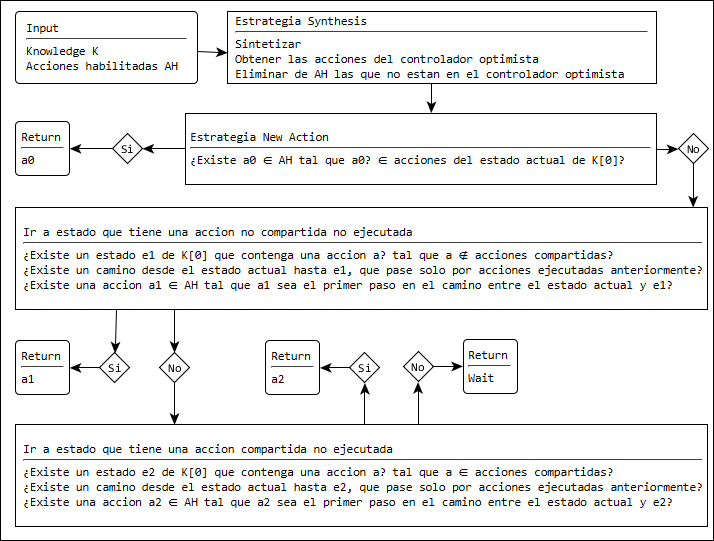
\includegraphics[scale=0.8]{Imagenes/Algoritmo/Algoritmo_elegir_2.png}
  \caption{Algoritmo de la estrategia Optimista - Nueva acción.}
  \label{fig:Algoritmo_elegir_2}
\end{figure}

\begin{algorithm}
\begin{algorithmic}
\REQUIRE MTS Knowledge, {Accion} Acciones habilitadas
\ENSURE Una accion que pertenece a Acciones habilitadas o Wait
\STATE Controlador optimista = Sintetizar(Knowledge)
\STATE Acciones del controlador optimista = obtener acciones habilitadas(Controlador optimista)
\STATE Acciones habilitadas = Acciones habilitadas $\cap$ Acciones del controlador optimista
\STATE Acciones habilitadas no ejecutadas = Acciones habilitadas $\cap$ acciones posibles(estado actual(Knowledge))
\IF{Acciones habilitadas no ejecutadas != $\emptyset$}
\RETURN Acciones habilitadas no ejecutadas[0]
\ELSE
\FOR{Estado $\in$ Estados(Knowledge)}
\IF{Estado == Estado inicial}
\STATE continue
\ENDIF
\STATE Acciones posibles no compartidas = acciones posibles no compartidas(Estado)
\IF{Acciones posibles no compartidas != $\emptyset$}
\STATE Controlador al estado = sintetizar para encontrar camino(Knowledge, Estado)
\STATE Acciones del controlador al estado = obtener acciones habilitadas(Controlador al estado)
\STATE Acciones habilitadas que llevan al estado = Acciones habilitadas $\cap$ Acciones del controlador al estado
\IF{Acciones habilitadas que llevan al estado != $\emptyset$}
\RETURN Acciones habilitadas que llevan al estado[0]
\ENDIF
\ENDIF
\ENDFOR
\FOR{Estado $\in$ Estados(Knowledge)}
\IF{Estado == Estado inicial}
\STATE continue
\ENDIF
\STATE Acciones posibles compartidas = acciones posibles compartidas(Estado)
\IF{Acciones posibles compartidas != $\emptyset$}
\STATE Controlador al estado = sintetizar para encontrar camino(Knowledge, Estado)
\STATE Acciones del controlador al estado = obtener acciones habilitadas(Controlador al estado)
\STATE Acciones habilitadas que llevan al estado = Acciones habilitadas $\cap$ Acciones del controlador al estado
\IF{Acciones habilitadas que llevan al estado != $\emptyset$}
\RETURN Acciones habilitadas que llevan al estado[0]
\ENDIF
\ENDIF
\ENDFOR
\RETURN Wait
\ENDIF
\end{algorithmic}
\caption{Algoritmo de la estrategia Optimista - Nueva acción}
\end{algorithm}

\newpage

\section{Ejecución}

\begin{figure}[H]
  \centering
    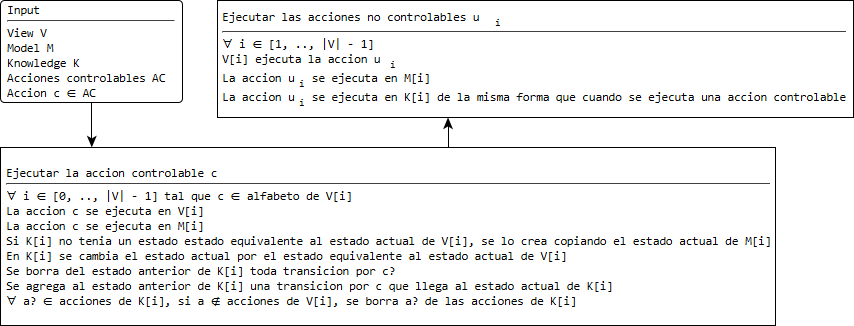
\includegraphics[width=1.0\textwidth]{Imagenes/Algoritmo/Algoritmo_ejecutar.png}
  \caption{Algoritmo de ejecución.}
  \label{fig:Algoritmo_ejecutar}
\end{figure}

\begin{algorithm}
\begin{algorithmic}
\REQUIRE \{LTS\} View, \{MTS\} Model, MTS Knowledge, {Accion} Acciones controlables, Accion Acción a ejecutar
\FOR{i = 0; i $<$ $|$View$|$; i++}
\IF{Acción a ejecutar $\notin$ Acciones(View[i])}
\STATE continue
\ENDIF
\STATE ejecutar(Accion acción a ejecutar, View[i])
\STATE ejecutar(Accion acción a ejecutar, Model[i])
\IF{Knowledge[i] == null}
\STATE Knowledge[i] = Model[i]
\ENDIF
\STATE Actualizar estado actual(Knowledge[i], View[i])
\STATE Eliminar transicion posible(Knowledge[i], Acción a ejecutar)
\STATE Agregar transicion(Knowledge[i], Acción a ejecutar)
\FOR{Accion posible in Acciones posibles(Knowledge[i])}
\IF{Accion posible $\notin$ Acciones posibles(View[i])}
\STATE Eliminar accion(Knowledge[i], Accion posible)
\ENDIF
\ENDFOR
\ENDFOR
\FOR{i = 1; i $<$ $|$View$|$; i++}
\STATE Ejecutar accion no controlable(View[i])
\STATE Ejecutar accion no controlable(Model[i])
\STATE Ejecutar accion no controlable(Knowledge[i])
\ENDFOR
\end{algorithmic}
\caption{Algoritmo de ejecución}
\end{algorithm}

Al ejecutar la acción elegida, el robot puede, o no, cambiar de ubicación en el entorno. Esto implica un cambio en el estado actual del primer componente tanto 
de \textbf{View}, como de \textbf{Model} y \textbf{Knowledge}. El primer componente de \textbf{Knowledge} también puede cambiar su estructura, refinando el MTS, 
como consecuencia de la nueva información aportada por los sensores del robot en su nueva ubicación.

Si es la primera vez que el robot se encuentra en la ubicación actual, se va a agregar un nuevo estado en el primer componente de \textbf{Knowledge}, en el que todas 
sus acciones se dirigen hacia \textit{La nube}. En caso de haber ejecutado una acción que se dirigía hacia \textit{La nube}, ahora podemos observar a que ubicación 
en el entorno nos lleva, por lo cual vamos a poder transformar en nuestro modelo dicha acción en una acción requerida que va hacia el estado correspondiente 
a la ubicación actual.

Luego de ejecutar la acción elegida, hay que ejecutar las acciones ejecutadas por los agentes externos. Los cambios en los agentes externos afectan el estado actual 
de las restantes componentes de \textbf{View}, \textbf{Model} y \textbf{Knowledge}, y la estructura de las restantes componentes de \textbf{Knowledge}. El proceso se 
realiza en la forma descripta por la figura 3.4.

\section{Ciclo de exploración}

\begin{figure}[H]
  \centering
    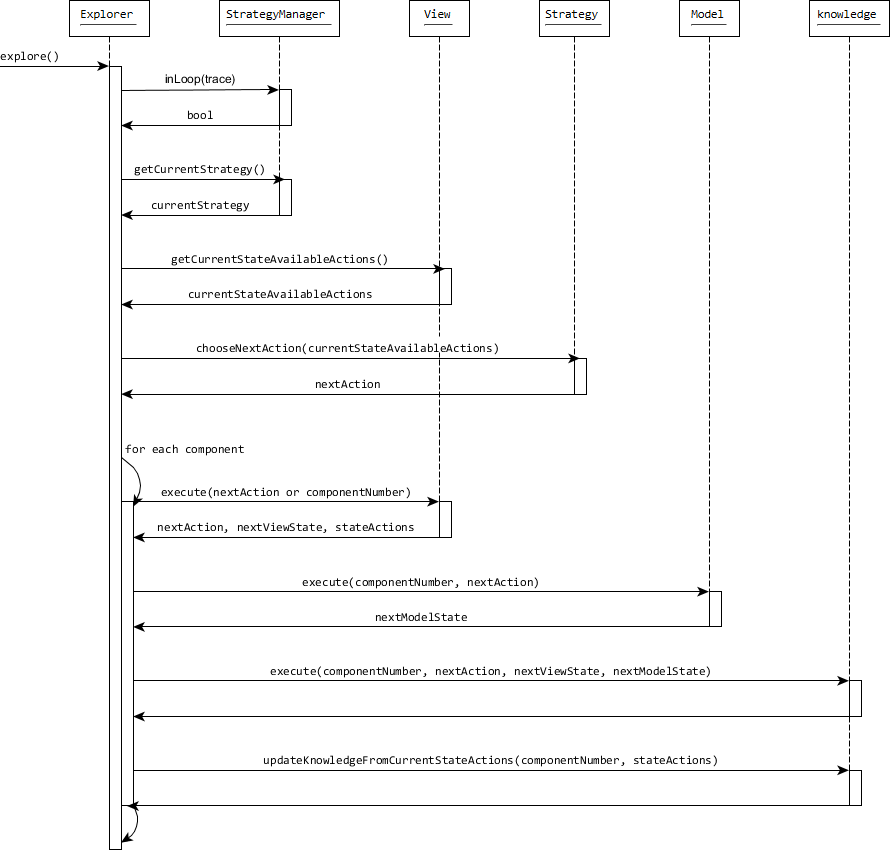
\includegraphics[width=1.0\textwidth]{Imagenes/Algoritmo/Secuencia_explorar.png}
  \caption{Diagrama de secuencia.}
  \label{fig:Secuencia_explorar}
\end{figure}

La figura 3.5 nos muestra cómo interactúan los diferentes objetos durante un ciclo de exploración.

Lo primero que hacemos es comprobar que la estrategia actual no haya entrado en un ciclo, ya que de no visitar estados nuevos no puede aportar información nueva.

En caso de que la estrategia actual esté en un ciclo la reemplazamos por otra. Una vez que tenemos la estrategia adecuada, observamos mediante los sensores que 
acciones tenemos disponibles en la ubicación actual, con el estado actual de los agentes externos. Le pedimos a la estrategia que elija una acción entre las 
acciones disponibles.

Cuando tenemos definida la siguiente acción, necesitamos ejecutarla. Primero la ejecutamos en \textbf{View}. Al hacerlo podemos censar en qué ubicación nos 
encontramos y qué acciones tenemos disponibles.

Luego la ejecutamos en \textbf{Model}, para que su estado actual se corresponda al estado que modela al estado actual de \textbf{View}.

A continuación, ejecutamos la acción en \textbf{Knowledge}, y en caso de que la acción vaya a un nuevo estado, utilizamos como nuevo estado el estado actual 
de \textbf{Model} (En este nuevo estado todas las acciones se dirigen hacia \textit{La nube}).

Por último, tenemos que agregar a \textbf{Knowledge} la nueva información obtenida, eliminando de su estado actual las acciones que no están disponibles, y 
transformando la acción que acabamos de ejecutar en caso de que originalmente estuviera dirigida hacia \textit{La nube}.

Luego de ejecutar la acción elegida, hay que ejecutar las acciones elegidas por los agentes externos. Cada componente extra en nuestros modelos representa a un agente 
externo, por lo tanto, hay que realizarlo una vez por componente. El proceso es el mismo que al ejecutar la acción elegida por nosotros, la única diferencia es que 
nosotros no elegimos la acción a ejecutar. Al hacer esto reflejamos el cambio en los agentes externos durante de tiempo que nos toma ejecutar nuestra acción.
\chapter{Resultados}

A continuación, vamos a plantear algunos casos de estudio para analizar en detalle el comportamiento del algoritmo.

\section{Laberinto de 25 posiciones}

El primer entorno que presentamos es un laberinto de 25 posiciones. En cada posición el robot puede tener hasta 4 
acciones disponibles, las cuales son norte, sur, este y oeste. El entorno no tiene agentes externos. El objetivo de 
este caso de estudio es ver como el robot encuentra la salida en un laberinto complejo sin información previa.

\begin{figure}[H]
	\centering
		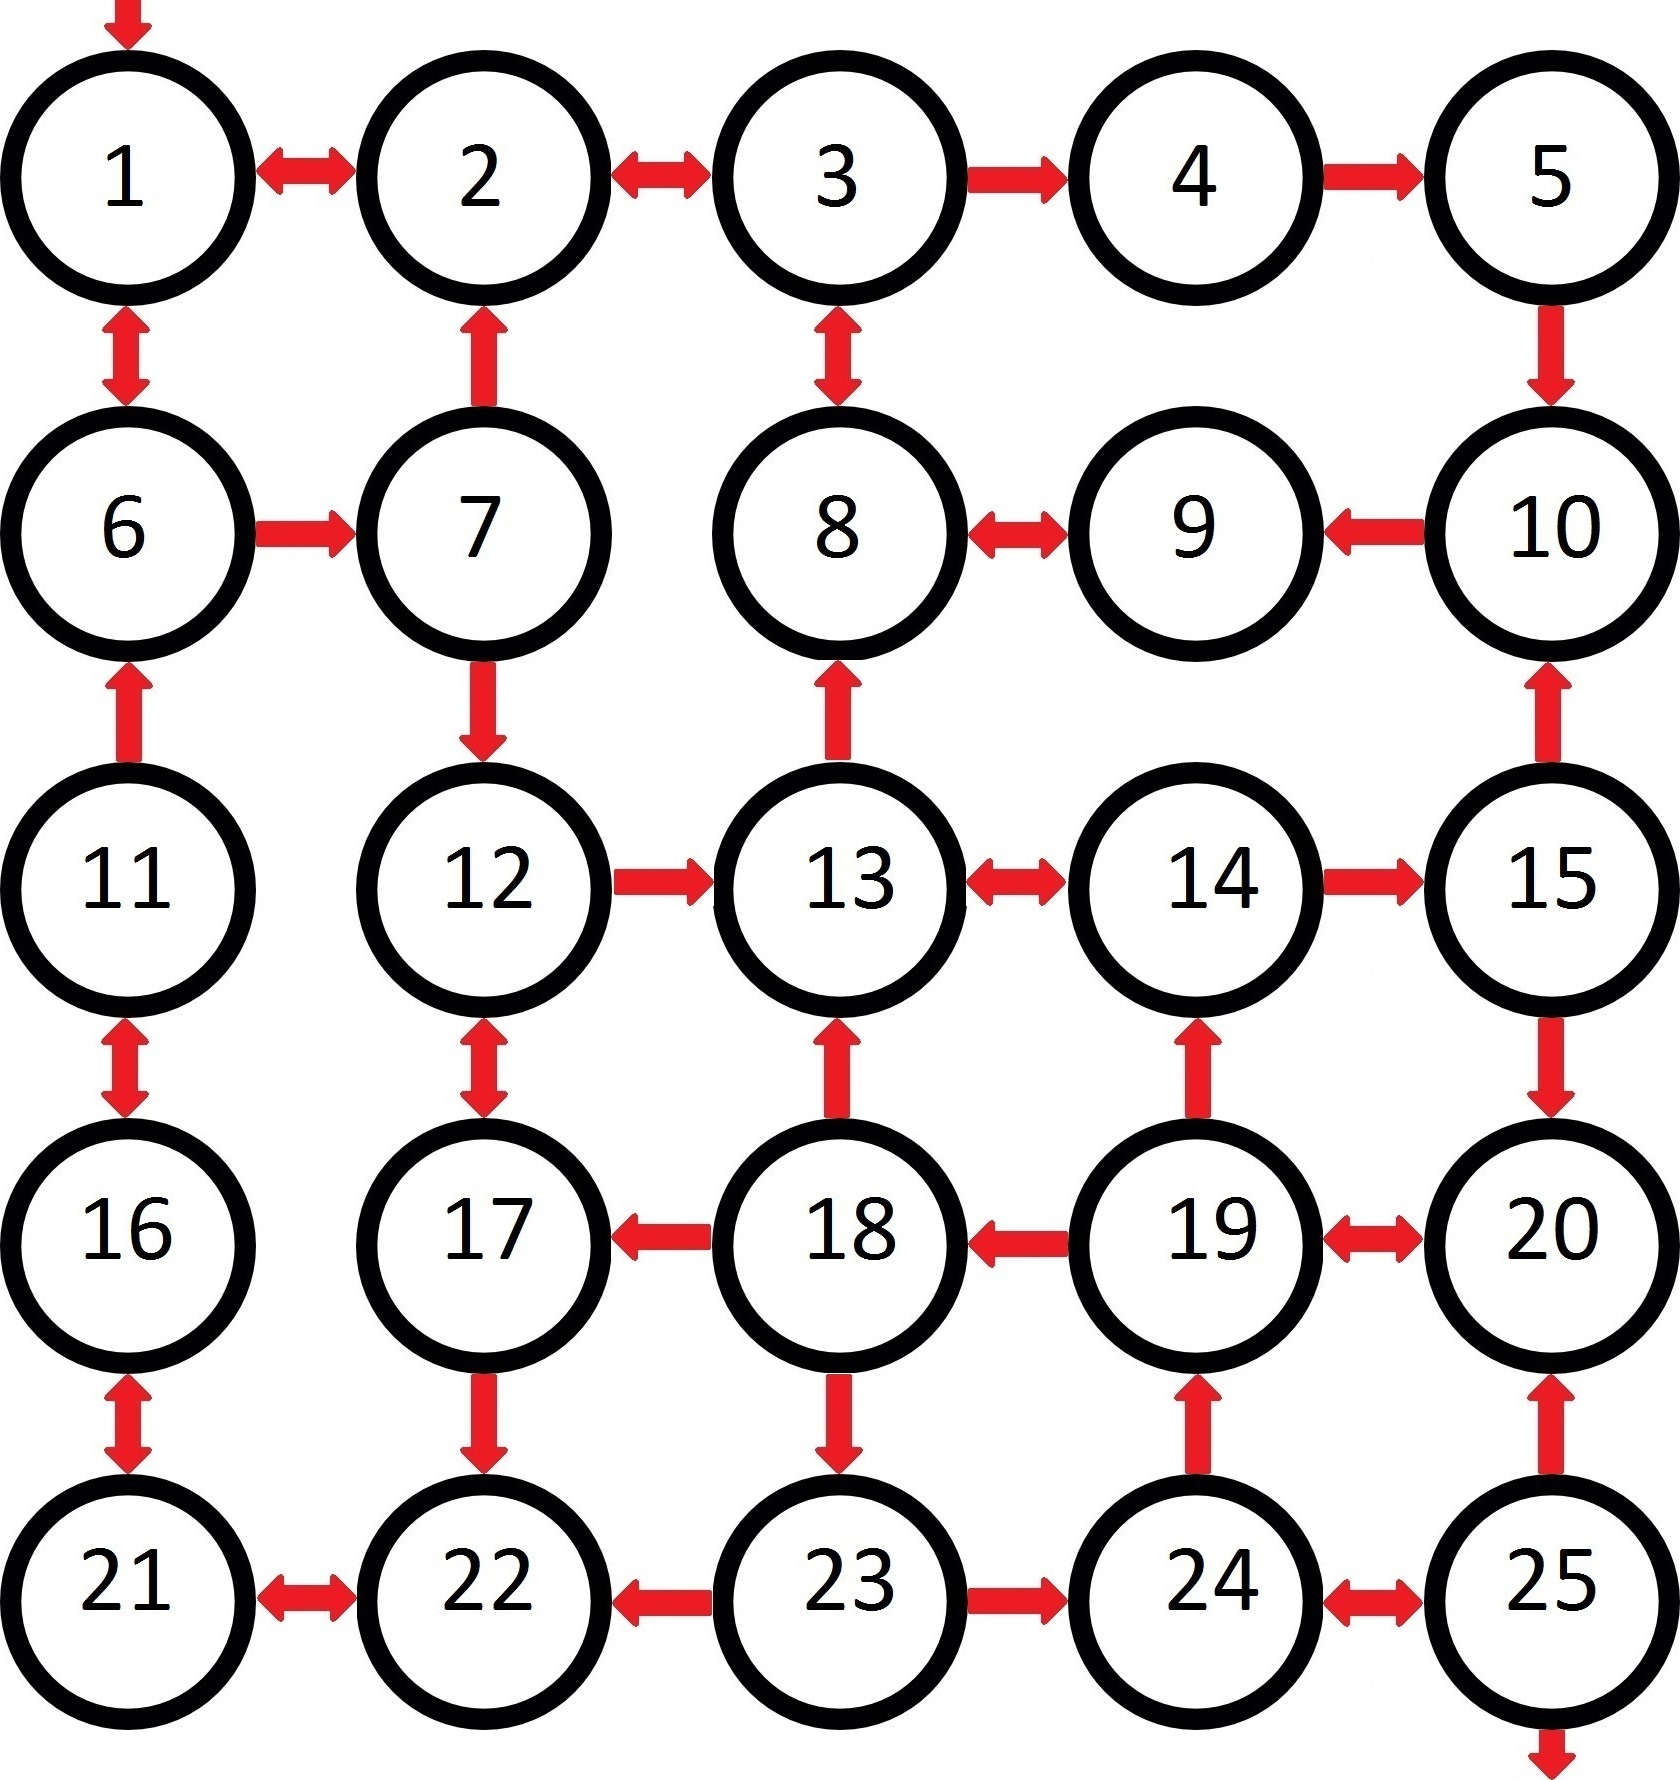
\includegraphics[scale=0.2]{Imagenes/Laberintos/25.jpg}
	\caption{Laberinto de 25 posiciones.}
	\label{fig:25}
\end{figure}

\newpage
\subsection{Especificación en MTSA}

\begin{Code}[commandchars=&\[\]]
&fvtextcolor[0000A0][VIEW] = &fvtextcolor[0000A0][P01],
&fvtextcolor[0000A0][P01]  = (sur   -> &fvtextcolor[0000A0][P06] | este  -> &fvtextcolor[0000A0][P02]),
&fvtextcolor[0000A0][P02]  = (este  -> &fvtextcolor[0000A0][P03] | oeste -> &fvtextcolor[0000A0][P01]),
&fvtextcolor[0000A0][P03]  = (sur   -> &fvtextcolor[0000A0][P08] | este  -> &fvtextcolor[0000A0][P04] | oeste -> &fvtextcolor[0000A0][P02]),
&fvtextcolor[0000A0][P04]  = (este  -> &fvtextcolor[0000A0][P05]),
&fvtextcolor[0000A0][P05]  = (sur   -> &fvtextcolor[0000A0][P10]),
&fvtextcolor[0000A0][P06]  = (norte -> &fvtextcolor[0000A0][P01] | este  -> &fvtextcolor[0000A0][P07]),
&fvtextcolor[0000A0][P07]  = (norte -> &fvtextcolor[0000A0][P02] | sur   -> &fvtextcolor[0000A0][P12]),
&fvtextcolor[0000A0][P08]  = (norte -> &fvtextcolor[0000A0][P03] | este  -> &fvtextcolor[0000A0][P09]),
&fvtextcolor[0000A0][P09]  = (oeste -> &fvtextcolor[0000A0][P08]),
&fvtextcolor[0000A0][P10]  = (oeste -> &fvtextcolor[0000A0][P09]),
&fvtextcolor[0000A0][P11]  = (norte -> &fvtextcolor[0000A0][P06] | sur   -> &fvtextcolor[0000A0][P16]),
&fvtextcolor[0000A0][P12]  = (sur   -> &fvtextcolor[0000A0][P17] | este  -> &fvtextcolor[0000A0][P13]),
&fvtextcolor[0000A0][P13]  = (norte -> &fvtextcolor[0000A0][P08] | este  -> &fvtextcolor[0000A0][P14]),
&fvtextcolor[0000A0][P14]  = (este  -> &fvtextcolor[0000A0][P15] | oeste -> &fvtextcolor[0000A0][P13]),
&fvtextcolor[0000A0][P15]  = (norte -> &fvtextcolor[0000A0][P10] | sur   -> &fvtextcolor[0000A0][P20]),
&fvtextcolor[0000A0][P16]  = (norte -> &fvtextcolor[0000A0][P11] | sur   -> &fvtextcolor[0000A0][P21]),
&fvtextcolor[0000A0][P17]  = (norte -> &fvtextcolor[0000A0][P12] | sur   -> &fvtextcolor[0000A0][P22]),
&fvtextcolor[0000A0][P18]  = (norte -> &fvtextcolor[0000A0][P13] | sur   -> &fvtextcolor[0000A0][P23] | oeste -> &fvtextcolor[0000A0][P17]),
&fvtextcolor[0000A0][P19]  = (norte -> &fvtextcolor[0000A0][P14] | este  -> &fvtextcolor[0000A0][P20] | oeste -> &fvtextcolor[0000A0][P18]),
&fvtextcolor[0000A0][P20]  = (oeste -> &fvtextcolor[0000A0][&fvtextcolor[0000A0][P19]]),
&fvtextcolor[0000A0][P21]  = (norte -> &fvtextcolor[0000A0][P16] | este  -> &fvtextcolor[0000A0][P22]),
&fvtextcolor[0000A0][P22]  = (oeste -> &fvtextcolor[0000A0][P21]),
&fvtextcolor[0000A0][P23]  = (este  -> &fvtextcolor[0000A0][P24] | oeste -> &fvtextcolor[0000A0][P22]),
&fvtextcolor[0000A0][P24]  = (norte -> &fvtextcolor[0000A0][&fvtextcolor[0000A0][P19]] | este  -> &fvtextcolor[0000A0][P25]),
&fvtextcolor[0000A0][P25]  = (norte -> &fvtextcolor[0000A0][P20] | oeste -> &fvtextcolor[0000A0][P24] | salir -> &fvtextcolor[0000A0][P25]).

&fvtextcolor[0000A0][MODEL] = (norte? -> &fvtextcolor[0000A0][MODEL] | sur?   -> &fvtextcolor[0000A0][MODEL] | este? -> &fvtextcolor[0000A0][MODEL] | 
         oeste? -> &fvtextcolor[0000A0][MODEL] | salir? -> &fvtextcolor[0000A0][MODEL]).

&fvtextcolor[0000FF][set] &fvtextcolor[0000A0][Controllable_25] = {norte, sur, este, oeste, salir}
&fvtextcolor[0000FF][fluent] &fvtextcolor[0000A0][F_Salir]      = <salir, &fvtextcolor[0000A0][Controllable_25]\{salir}>
&fvtextcolor[0000FF][assert] &fvtextcolor[0000A0][A_Salir]      = &fvtextcolor[0000A0][F_Salir]

&fvtextcolor[0000FF][controllerSpec] &fvtextcolor[0000A0][GOAL_25] = {
    liveness     = {&fvtextcolor[0000A0][A_Salir]}
    controllable = {&fvtextcolor[0000A0][Controllable_25]}
}

&fvtextcolor[0000FF][exploration] &fvtextcolor[0000A0][M25] = {
    environment = {&fvtextcolor[0000A0][VIEW]},
    model       = {&fvtextcolor[0000A0][MODEL]},
    goal        = {&fvtextcolor[0000A0][GOAL_25]}
}
\end{Code}

\subsection{Estrategia Optimista}

El robot logra salir del laberinto en 79 pasos, pasando en promedio 3.16 veces por cada posición.

\begin{figure}[H]
	\centering
		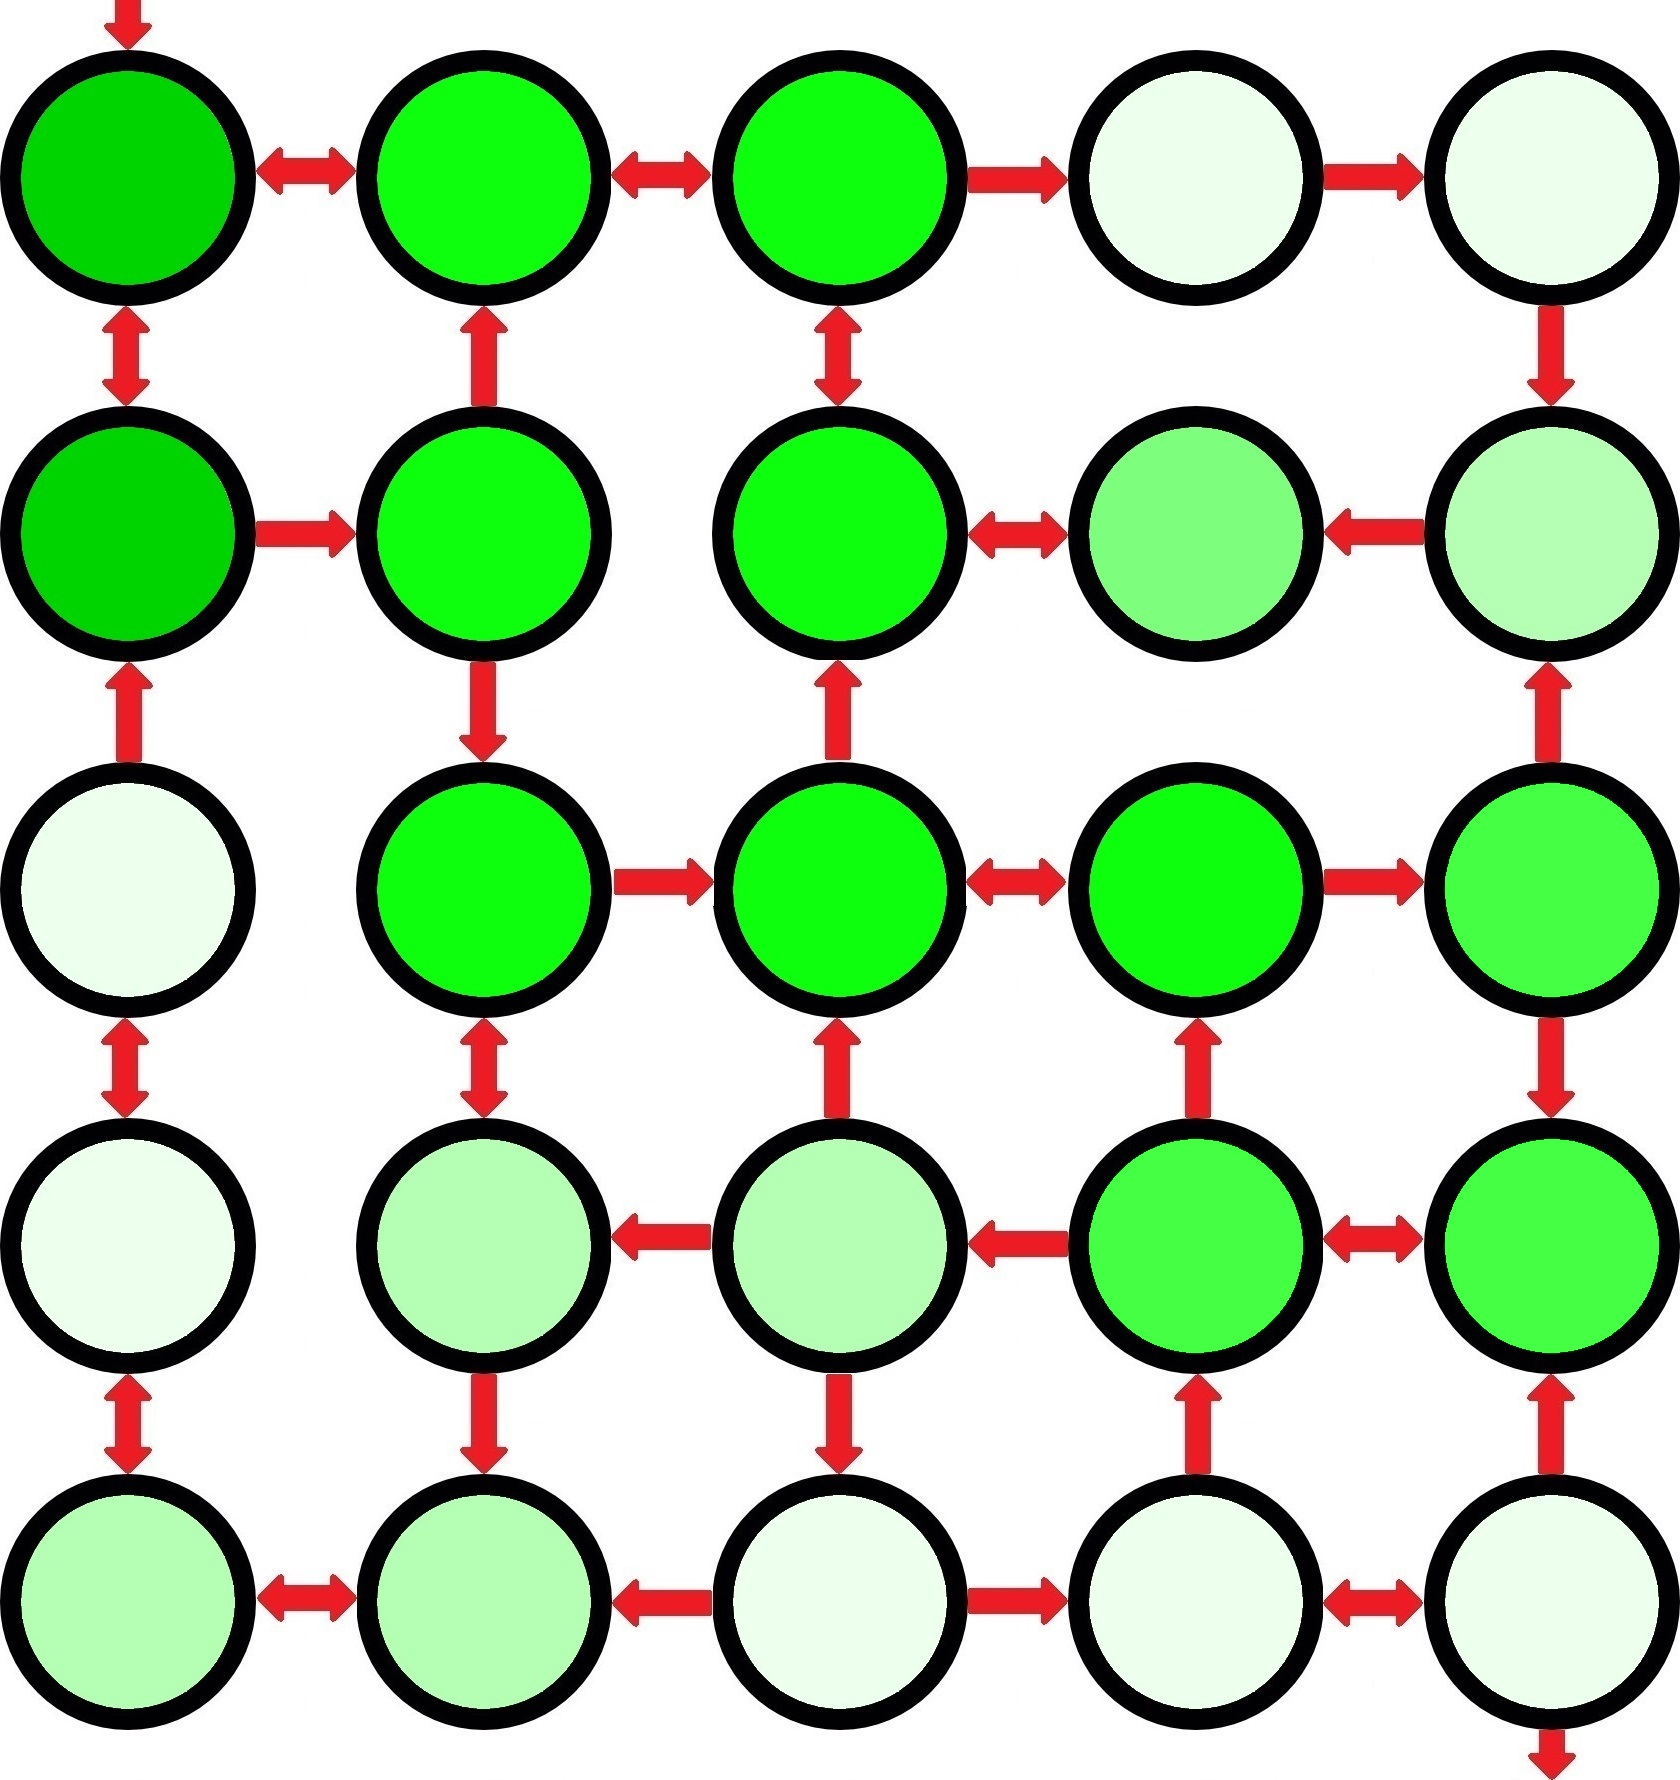
\includegraphics[scale=0.2]{Imagenes/Laberintos/25_calor_optimista.jpg}
	\caption{Mapa de calor del robot en el laberinto de 25 posiciones utilizando la estrategia Optimista.}
	\label{fig:25_calor}
\end{figure}

En el siguiente video \url{https://youtu.be/KakVlfLrIx4} podemos observar, paso a paso, como se mueve el
robot a través del entorno mientras realiza la exploración.

\clearpage

\subsubsection{Análisis de los modelos}

Para lograr dar una respuesta sobre si es posible o no garantizar el cumplimiento del objetivo fue necesario 
explorar el entorno casi por completo. Únicamente siete acciones no fueron ejecutadas.

\begin{figure}[H]
	\centering
		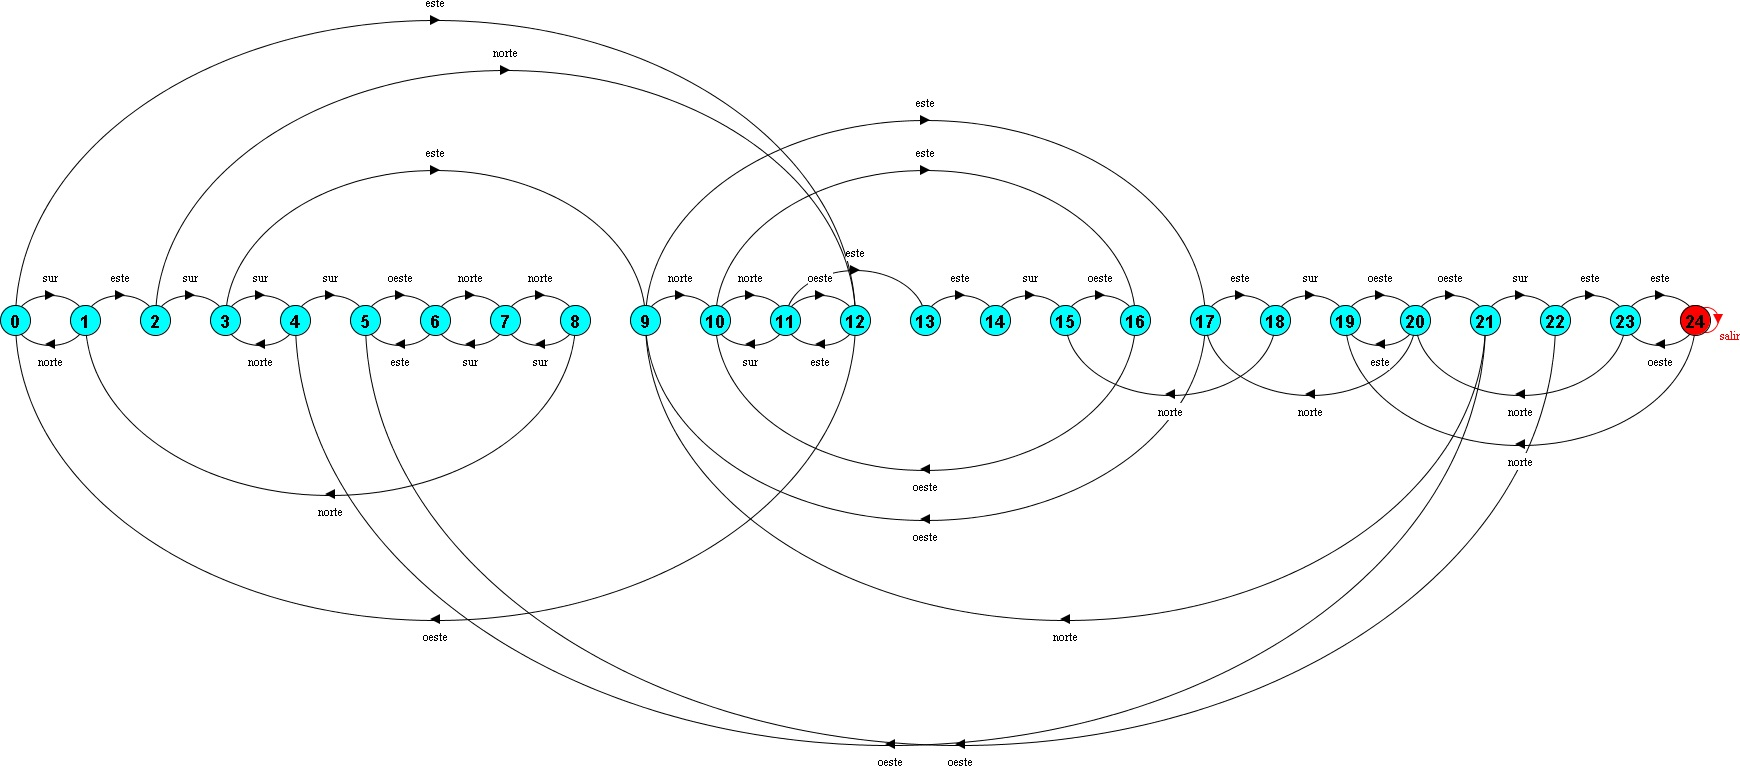
\includegraphics[width=1.0\textwidth]{Imagenes/Laberintos/25_view.jpg}
	\caption{LTS que representa al mapa del laberinto de 25 posiciones.}
	\label{fig:25_view}
\end{figure}

\begin{figure}[H]
	\centering
		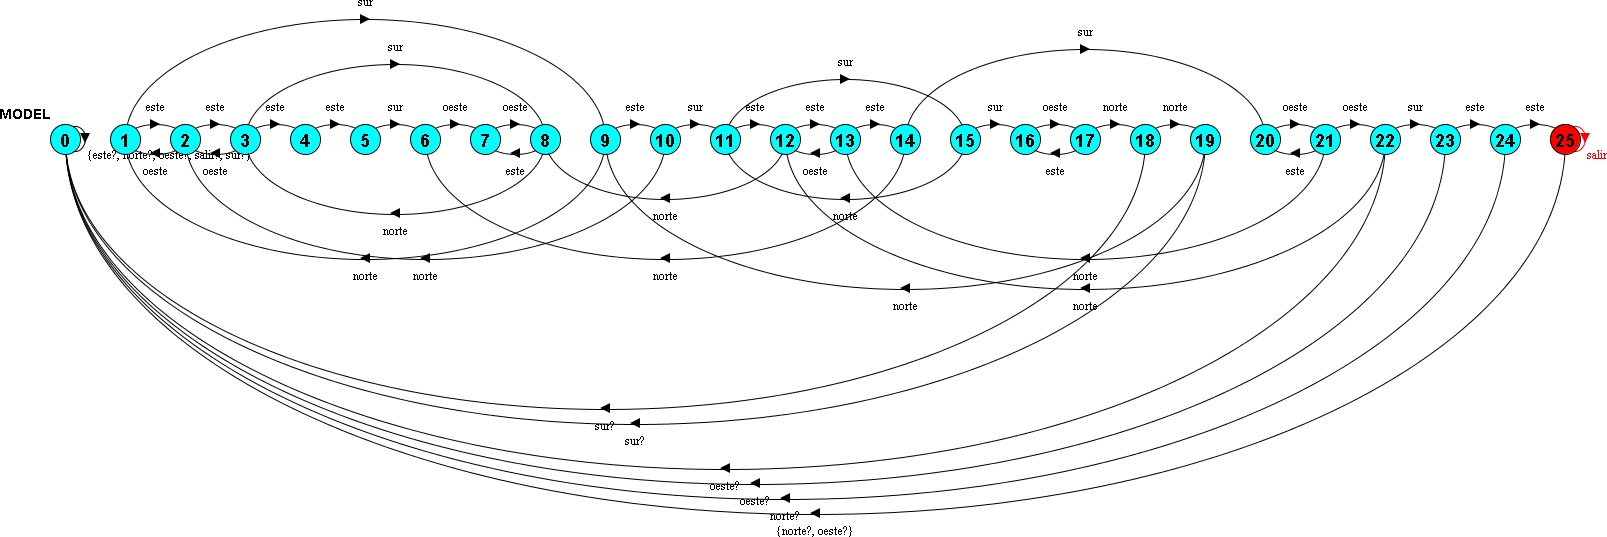
\includegraphics[width=1.0\textwidth]{Imagenes/Laberintos/25_knowledge_optimista.jpg}
	\caption{MTS que representa al conocimiento adquirido sobre el laberinto de 25 posiciones utilizando la estrategia Optimista.}
	\label{fig:25_knowledge}
\end{figure}

\clearpage

\subsection{Estrategia Optimista - Nueva acción}

En este caso de prueba, el modelo de conocimiento con el cual contamos al inicio de la exploración, no aporta información sobre
zonas inseguras, por lo cual las estrategias Nueva acción y Optimista - Nueva acción obtienen exactamente el mismo resultado.

\subsubsection{Análisis preliminar}

El robot logra salir del laberinto en 116 pasos, pasando en promedio 4.64 veces por cada posición. 
Podemos observar a simple vista que las posiciones más visitadas forman parte del camino hacia la salida.

\begin{figure}[H]
	\centering
		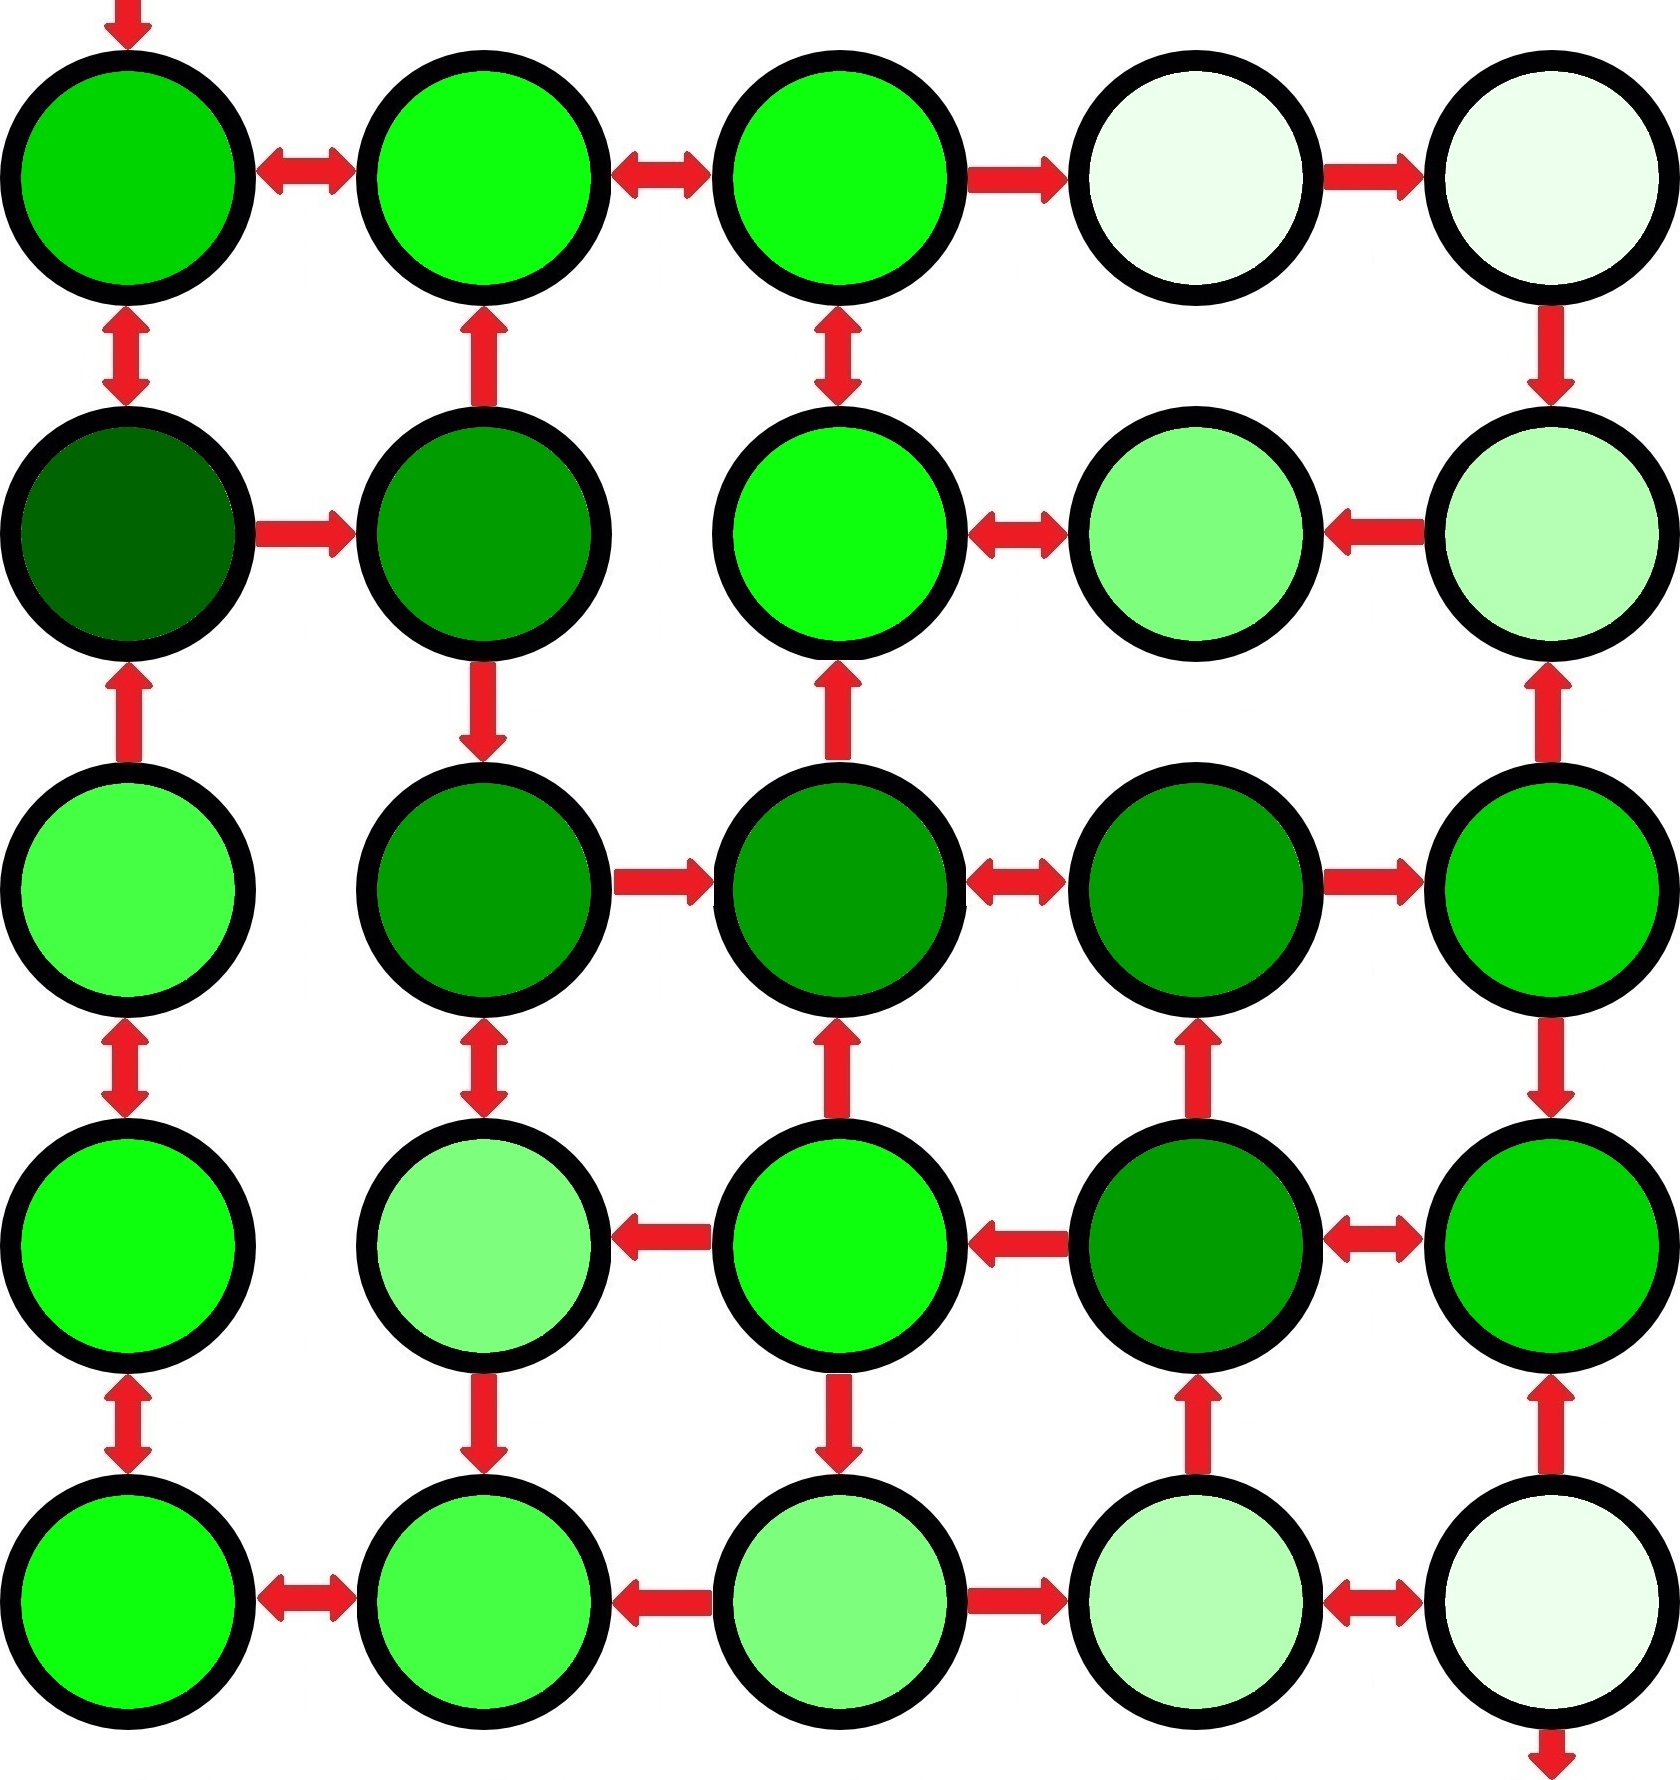
\includegraphics[scale=0.2]{Imagenes/Laberintos/25_calor.jpg}
	\caption{Mapa de calor del robot en el laberinto de 25 posiciones utilizando la estrategia Optimista - Nueva acción.}
	\label{fig:25_calor}
\end{figure}

En el siguiente video \url{https://youtu.be/8XwPYquCUB4} podemos observar, paso a paso, como se mueve el
robot a través del entorno mientras realiza la exploración. El video nos permite ver de una forma más
clara que regiones explora primero, y como va aprendiendo caminos que le permiten llegar a posiciones prometedoras
para la exploración.

\clearpage

\subsubsection{Análisis de los modelos}

Para lograr dar una respuesta sobre si es posible o no garantizar el cumplimiento del objetivo fue necesario 
explorar el entorno casi por completo. Las únicas dos acciones no ejecutadas fueron norte y oeste desde la posición 
final, por lo cual en el modelo del conocimiento van hacia \textit{La nube}.

\begin{figure}[H]
	\centering
		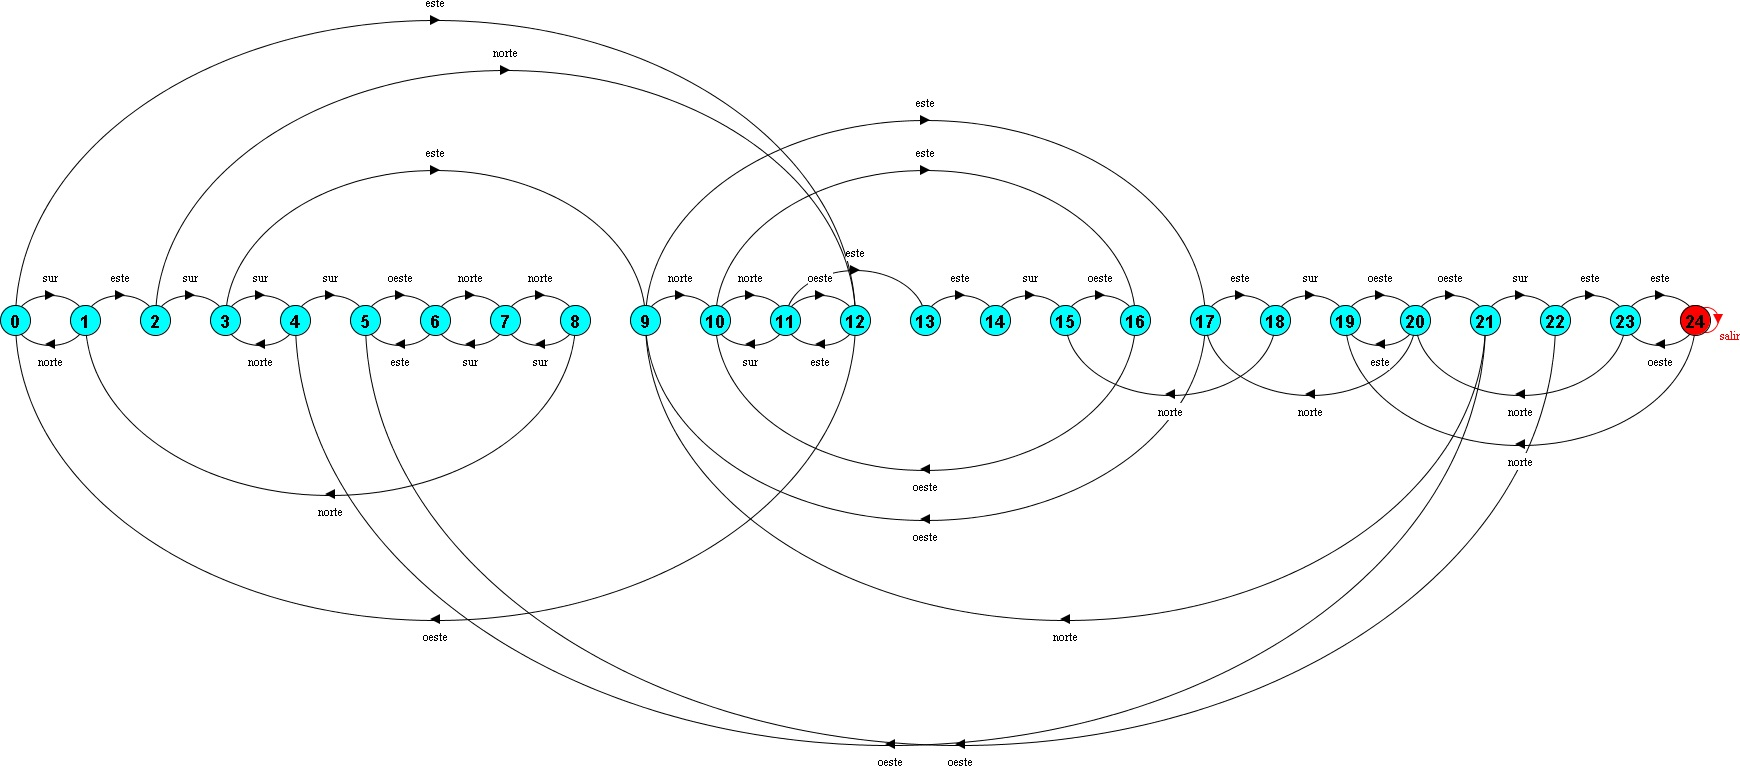
\includegraphics[width=1.0\textwidth]{Imagenes/Laberintos/25_view.jpg}
	\caption{LTS que representa al mapa del laberinto de 25 posiciones.}
	\label{fig:25_view}
\end{figure}

\begin{figure}[H]
	\centering
		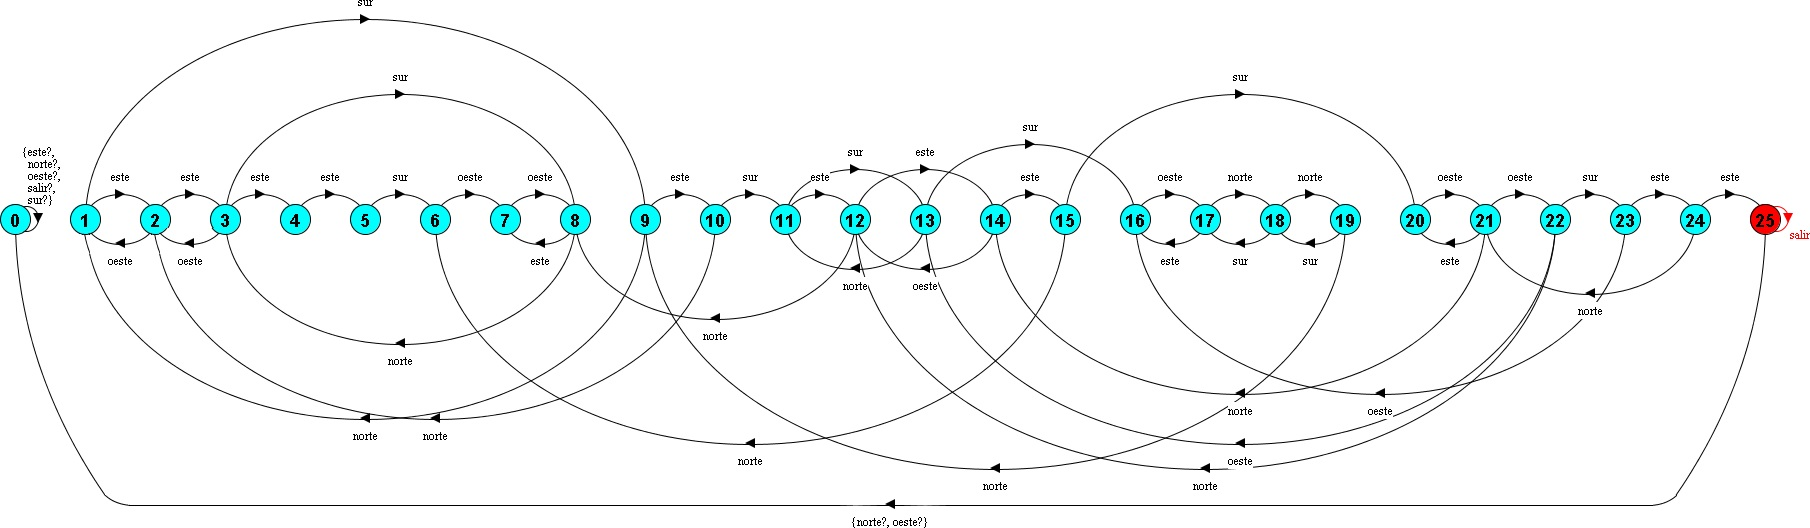
\includegraphics[width=1.0\textwidth]{Imagenes/Laberintos/25_knowledge.jpg}
	\caption{MTS que representa al conocimiento adquirido sobre el laberinto de 25 posiciones utilizando la estrategia Optimista - Nueva acción.}
	\label{fig:25_knowledge}
\end{figure}

\clearpage

\subsection{Variantes}

Si eliminamos la acción salir, el robot descubre que el laberinto no tiene salida en 122 pasos, formando un modelo 
de conocimiento de dos componentes conexas, en cual una componente conexa es bisimilar al LTS que representa al mapa, 
mientras que la otra componente conexa \textit{La nube}.

\vspace{\baselineskip}
Si modificamos el mapa para que la acción salir se encuentre en \textcolor[HTML]{0000A0}{P08} en vez de encontrarse 
en \textcolor[HTML]{0000A0}{P25}, el robot logra salir del laberinto en solamente 9 pasos, siendo su modelo del conocimiento 
mucho más reducido que el modelo del mapa.

\begin{figure}[H]
	\centering
		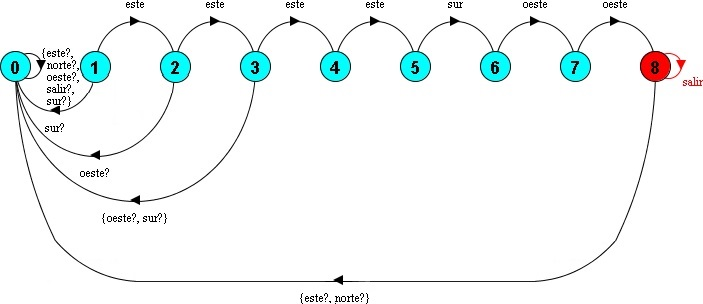
\includegraphics[width=1.0\textwidth]{Imagenes/Laberintos/25_knowledge_alternativo.jpg}
	\caption{MTS que representa al conocimiento adquirido sobre el laberinto de 25 posiciones con salida en la posición 8.}
	\label{fig:25_knowledge_alternativo}
\end{figure}

Tanto utilizando la estrategia Optimista como la estrategia Optimista - Nueva acción, el resultado es el mismo con ambas variantes.

\clearpage

\section{Zonas inseguras}

En este ejemplo veremos como la estrategia Optimista utiliza nuestro conocimiento previo para evitar las zonas inseguras.

\begin{figure}[H]
	\centering
		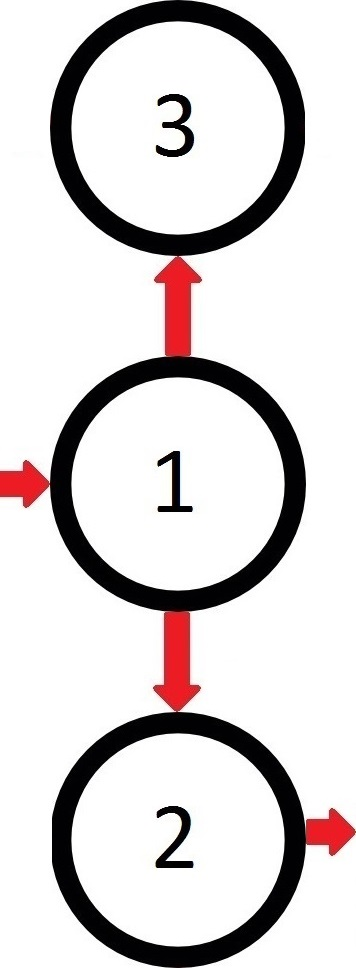
\includegraphics[scale=0.2]{Imagenes/Laberintos/unsafe.jpg}
	\caption{Laberinto con zona insegura.}
	\label{fig:unsafe}
\end{figure}

\subsection{Especificación en MTSA}

\begin{Code}[commandchars=&\[\]]
&fvtextcolor[0000A0][VIEW]   = (sur    -> &fvtextcolor[0000A0][GANAR] | norte -> &fvtextcolor[0000A0][PERDER]),
&fvtextcolor[0000A0][GANAR]  = (ganar  -> &fvtextcolor[0000A0][GANAR]),
&fvtextcolor[0000A0][PERDER] = (perder -> &fvtextcolor[0000A0][PERDER]).

&fvtextcolor[0000A0][MODEL_CON_INFO] = (sur?    -> &fvtextcolor[0000A0][MODEL_GANAR]    | norte?  -> &fvtextcolor[0000A0][MODEL_PERDER]  | 
                  ganar?  -> &fvtextcolor[0000A0][MODEL_CON_INFO] | perder? -> &fvtextcolor[0000A0][MODEL_CON_INFO]),
&fvtextcolor[0000A0][MODEL_GANAR]    = (sur?    -> &fvtextcolor[0000A0][MODEL_GANAR]    | norte?  -> &fvtextcolor[0000A0][MODEL_GANAR]   |
                  ganar?  -> &fvtextcolor[0000A0][MODEL_GANAR]),
&fvtextcolor[0000A0][MODEL_PERDER]   = (sur?    -> &fvtextcolor[0000A0][MODEL_PERDER]   | norte?  -> &fvtextcolor[0000A0][MODEL_PERDER]  | 
                  perder? -> &fvtextcolor[0000A0][MODEL_PERDER]).

&fvtextcolor[0000FF][set] &fvtextcolor[0000A0][Controllable_UNSAFE] = {norte, sur, ganar, perder}
&fvtextcolor[0000FF][fluent] &fvtextcolor[0000A0][F_Ganar]          = <ganar, &fvtextcolor[0000A0][Controllable_UNSAFE]\{ganar}>
&fvtextcolor[0000FF][assert] &fvtextcolor[0000A0][A_Ganar]          = &fvtextcolor[0000A0][F_Ganar]

&fvtextcolor[0000FF][controllerSpec] &fvtextcolor[0000A0][GOAL_UNSAFE] = {
    liveness     = {&fvtextcolor[0000A0][A_Ganar]}
    controllable = {&fvtextcolor[0000A0][Controllable_UNSAFE]}
}

&fvtextcolor[0000FF][exploration] &fvtextcolor[0000A0][UNSAFE] = {
    environment = {&fvtextcolor[0000A0][VIEW]},
    model       = {&fvtextcolor[0000A0][MODEL_CON_INFO]},
    goal        = {&fvtextcolor[0000A0][GOAL_UNSAFE]}
}
\end{Code}

\subsection{Análisis de los modelos}

\begin{figure}[H]
	\centering
		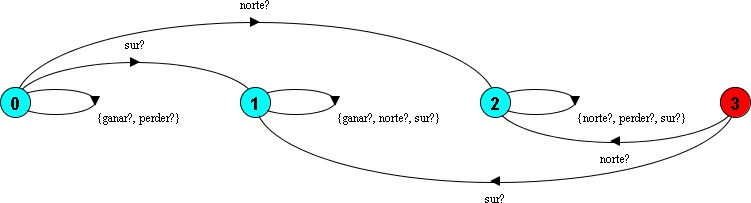
\includegraphics[width=1.0\textwidth]{Imagenes/Laberintos/unsafe_inicio.jpg}
	\caption{MTS que representa al conocimiento inicial sobre el laberinto con zona insegura.}
	\label{fig:unsafe_inicio}
\end{figure}

En la figura 4.7 podemos observar nuestro conocimiento sobre el entorno al iniciar la exploración. Los estados 0, 1 y 2 pertenecen a \textit{La nube}, 
el estado 3 es el estado inicial.

\begin{figure}[H]
	\centering
		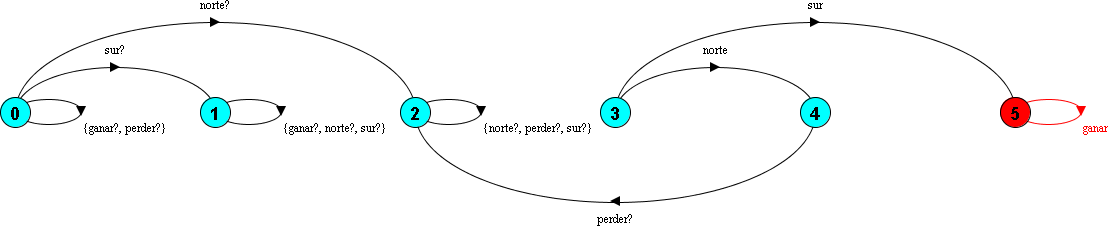
\includegraphics[width=1.0\textwidth]{Imagenes/Laberintos/unsafe_nueva_accion.png}
	\caption{MTS que representa al conocimiento adquirido sobre el laberinto con zona insegura, utilizando la estrategia Nueva Acción.}
	\label{fig:unsafe_nueva_accion}
\end{figure}

Si utilizamos la estrategia Nueva Acción, lo único que importa es elegir una acción nueva. En el caso de la figura 4.8, la estrategia eligió primero norte, 
llegando así a un estado sin salida. Fue necesario realizar un reset para luego elegir sur y llegar a un estado ganador.

\begin{figure}[H]
	\centering
		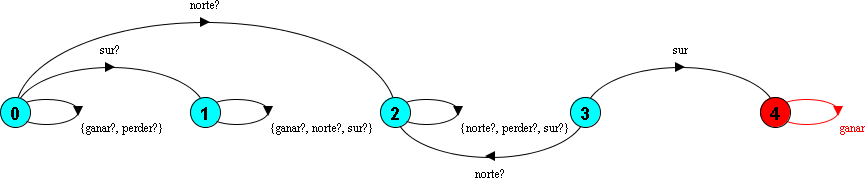
\includegraphics[width=1.0\textwidth]{Imagenes/Laberintos/unsafe_sintesis.png}
	\caption{MTS que representa al conocimiento adquirido sobre el laberinto con zona insegura, utilizando la estrategia Optimista - Nueva Acción.}
	\label{fig:unsafe_sintesis}
\end{figure}

En cambio, utilizando la estrategia Optimista u Optimista - Nueva Acción, por construcción, el controlador optimista evita las zonas inseguras. Al elegir la acción, 
se descarta norte, por lo cual el robot llega a un estado ganador sin la necesidad de realizar un reset, como puede observarse en la figura 4.9.

\clearpage

\section{Laberinto que baja}

En este ejemplo, el robot se puede mover libremente en forma horizontal, ya que si se mueve a izquierda o derecha, siempre puede regresar a la posición en la que estaba. 
Si el robot se mueve hacia abajo no puede volver a subir. La salida no se encuentra en el nivel inferior, por lo cual todos los estados del nivel inferior son estados perdedores.

\begin{figure}[H]
	\centering
		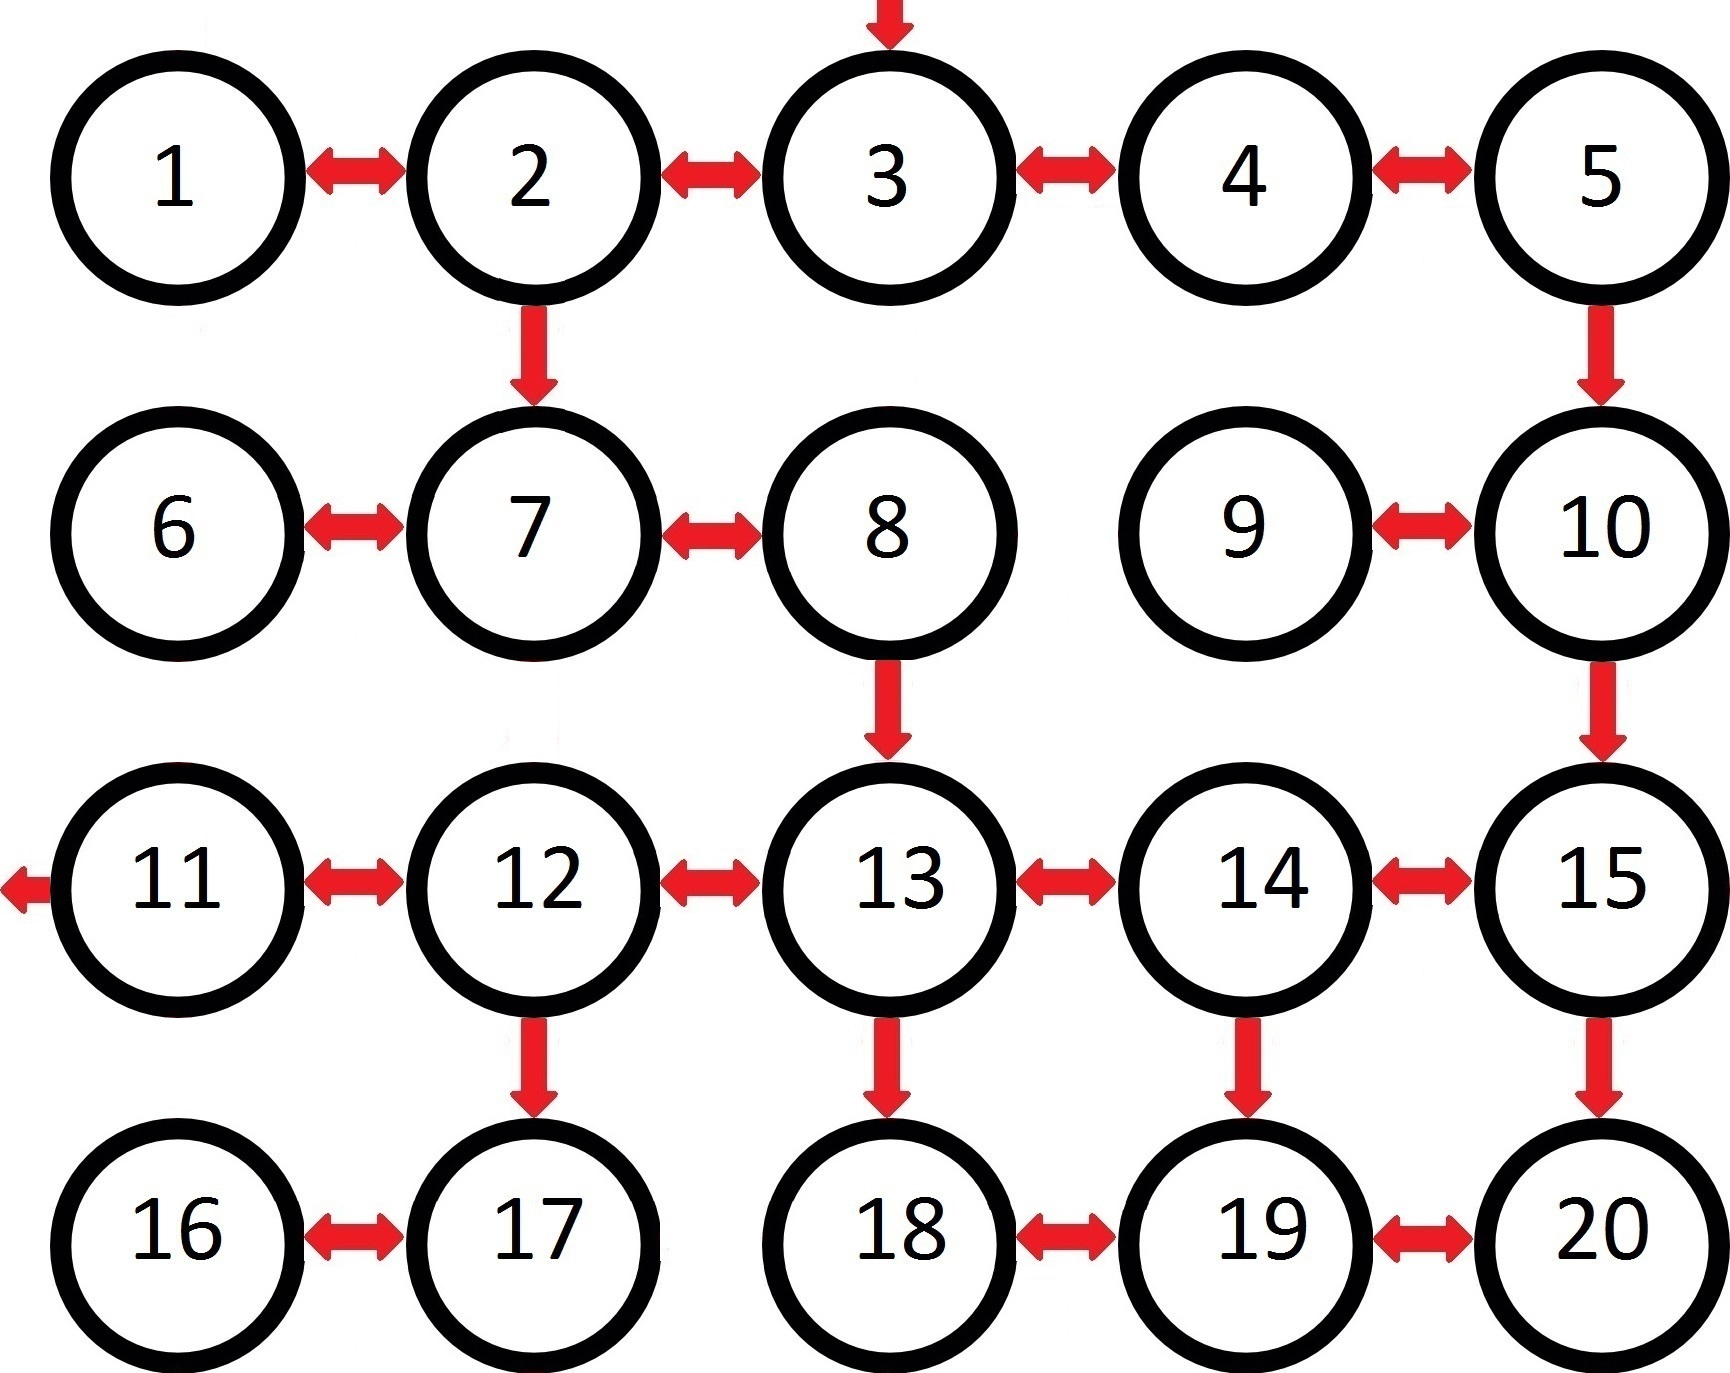
\includegraphics[scale=0.2]{Imagenes/Laberintos/Down.jpg}
	\caption{Laberinto que baja.}
	\label{fig:down}
\end{figure}

\subsection{Especificación en MTSA}

\begin{Code}[commandchars=&\[\]]
&fvtextcolor[0000A0][VIEW] = &fvtextcolor[0000A0][P03],
&fvtextcolor[0000A0][P01] = (este  -> &fvtextcolor[0000A0][P02]),
&fvtextcolor[0000A0][P02] = (sur   -> &fvtextcolor[0000A0][P07] | este  -> &fvtextcolor[0000A0][P03] | oeste -> &fvtextcolor[0000A0][P01]),
&fvtextcolor[0000A0][P03] = (este  -> &fvtextcolor[0000A0][P04] | oeste -> &fvtextcolor[0000A0][P02]),
&fvtextcolor[0000A0][P04] = (este  -> &fvtextcolor[0000A0][P05] | oeste -> &fvtextcolor[0000A0][P03]),
&fvtextcolor[0000A0][P05] = (sur   -> &fvtextcolor[0000A0][P10] | oeste -> &fvtextcolor[0000A0][P04]),
&fvtextcolor[0000A0][P06] = (este  -> &fvtextcolor[0000A0][P07]),
&fvtextcolor[0000A0][P07] = (este  -> &fvtextcolor[0000A0][P08] | oeste -> &fvtextcolor[0000A0][P06]),
&fvtextcolor[0000A0][P08] = (sur   -> &fvtextcolor[0000A0][P13] | oeste -> &fvtextcolor[0000A0][P07]),
&fvtextcolor[0000A0][P09] = (este  -> &fvtextcolor[0000A0][P10]),
&fvtextcolor[0000A0][P10] = (sur   -> &fvtextcolor[0000A0][P15] | oeste -> &fvtextcolor[0000A0][P09]),
&fvtextcolor[0000A0][P11] = (este  -> &fvtextcolor[0000A0][P12] | salir -> &fvtextcolor[0000A0][P11]),
&fvtextcolor[0000A0][P12] = (sur   -> &fvtextcolor[0000A0][P17] | este  -> &fvtextcolor[0000A0][P13] | oeste -> &fvtextcolor[0000A0][P11]),
&fvtextcolor[0000A0][P13] = (sur   -> &fvtextcolor[0000A0][P18] | este  -> &fvtextcolor[0000A0][P14] | oeste -> &fvtextcolor[0000A0][P12]),
&fvtextcolor[0000A0][P14] = (sur   -> &fvtextcolor[0000A0][P19] | este  -> &fvtextcolor[0000A0][P15] | oeste -> &fvtextcolor[0000A0][P13]),
&fvtextcolor[0000A0][P15] = (sur   -> &fvtextcolor[0000A0][P20] | oeste -> &fvtextcolor[0000A0][P14]),
&fvtextcolor[0000A0][P16] = (este  -> &fvtextcolor[0000A0][P17]),
&fvtextcolor[0000A0][P17] = (oeste -> &fvtextcolor[0000A0][P16]),
&fvtextcolor[0000A0][P18] = (este  -> &fvtextcolor[0000A0][P19]),
&fvtextcolor[0000A0][P19] = (este  -> &fvtextcolor[0000A0][P20] | oeste -> &fvtextcolor[0000A0][P18]),
&fvtextcolor[0000A0][P20] = (oeste -> &fvtextcolor[0000A0][P19]).

&fvtextcolor[0000A0][MODEL_CON_INFO] = &fvtextcolor[0000A0][CENTRO],
&fvtextcolor[0000A0][CENTRO]  = (sur?   -> &fvtextcolor[0000A0][CENTRO]  | este?  -> &fvtextcolor[0000A0][ESTE_1] | 
           oeste? -> &fvtextcolor[0000A0][OESTE_1] | salir? -> &fvtextcolor[0000A0][CENTRO]),
&fvtextcolor[0000A0][ESTE_1]  = (sur?   -> &fvtextcolor[0000A0][CENTRO]  | este?  -> &fvtextcolor[0000A0][ESTE_2] | 
           oeste  -> &fvtextcolor[0000A0][CENTRO]  | salir? -> &fvtextcolor[0000A0][ESTE_1]),
&fvtextcolor[0000A0][ESTE_2]  = (sur?   -> &fvtextcolor[0000A0][CENTRO]  | este?  -> &fvtextcolor[0000A0][ESTE_3] | 
           oeste  -> &fvtextcolor[0000A0][ESTE_1]  | salir? -> &fvtextcolor[0000A0][ESTE_2]),
&fvtextcolor[0000A0][ESTE_3]  = (sur?   -> &fvtextcolor[0000A0][CENTRO]  | este?  -> &fvtextcolor[0000A0][ESTE_4] | 
           oeste  -> &fvtextcolor[0000A0][ESTE_2]  | salir? -> &fvtextcolor[0000A0][ESTE_3]),
&fvtextcolor[0000A0][ESTE_4]  = (sur?   -> &fvtextcolor[0000A0][CENTRO]  | oeste  -> &fvtextcolor[0000A0][ESTE_3] | 
           salir? -> &fvtextcolor[0000A0][ESTE_4]),
&fvtextcolor[0000A0][OESTE_1] = (sur?   -> &fvtextcolor[0000A0][CENTRO]  | este   -> &fvtextcolor[0000A0][CENTRO]  | 
           oeste? -> &fvtextcolor[0000A0][OESTE_2] | salir? -> &fvtextcolor[0000A0][OESTE_1]),
&fvtextcolor[0000A0][OESTE_2] = (sur?   -> &fvtextcolor[0000A0][CENTRO]  | este   -> &fvtextcolor[0000A0][OESTE_1] | 
           oeste? -> &fvtextcolor[0000A0][OESTE_3] | salir? -> &fvtextcolor[0000A0][OESTE_2]),
&fvtextcolor[0000A0][OESTE_3] = (sur?   -> &fvtextcolor[0000A0][CENTRO]  | este   -> &fvtextcolor[0000A0][OESTE_2] | 
           oeste? -> &fvtextcolor[0000A0][OESTE_4] | salir? -> &fvtextcolor[0000A0][OESTE_3]),
&fvtextcolor[0000A0][OESTE_4] = (sur?   -> &fvtextcolor[0000A0][CENTRO]  | este   -> &fvtextcolor[0000A0][OESTE_3] | 
           salir? -> &fvtextcolor[0000A0][OESTE_4]).

&fvtextcolor[0000FF][set] &fvtextcolor[0000A0][Controllable_Down] = {sur, este, oeste, salir}
&fvtextcolor[0000FF][fluent] &fvtextcolor[0000A0][F_Salir]        = <salir, &fvtextcolor[0000A0][Controllable_Down]\{salir}>
&fvtextcolor[0000FF][assert] &fvtextcolor[0000A0][A_Salir]        = &fvtextcolor[0000A0][F_Salir]

&fvtextcolor[0000FF][controllerSpec] &fvtextcolor[0000A0][GOAL_Down] = {
    liveness     = {&fvtextcolor[0000A0][A_Salir]}
    controllable = {&fvtextcolor[0000A0][Controllable_Down]}
}

&fvtextcolor[0000FF][exploration] &fvtextcolor[0000A0][MDown] = {
    environment = {&fvtextcolor[0000A0][VIEW]},
    model       = {&fvtextcolor[0000A0][MODEL_CON_INFO]},
    goal        = {&fvtextcolor[0000A0][GOAL_Down]}
}
\end{Code}

\clearpage

\subsection{Análisis de los modelos}

Sabemos que:
\begin{itemize}

\item
Si podemos movernos una posición horizontalmente, también vamos a poder movernos una posición en la dirección contraria.

\item
Como máximo podemos movernos hasta cuatro veces en la misma dirección.

\item
Si bajamos, llegamos a una posición que cumple las dos condiciones antes mencionadas.

\end{itemize}

Vamos a utilizar como modelo del conocimiento inicial un MTS que represente estas tres condiciones.

\begin{figure}[H]
	\centering
		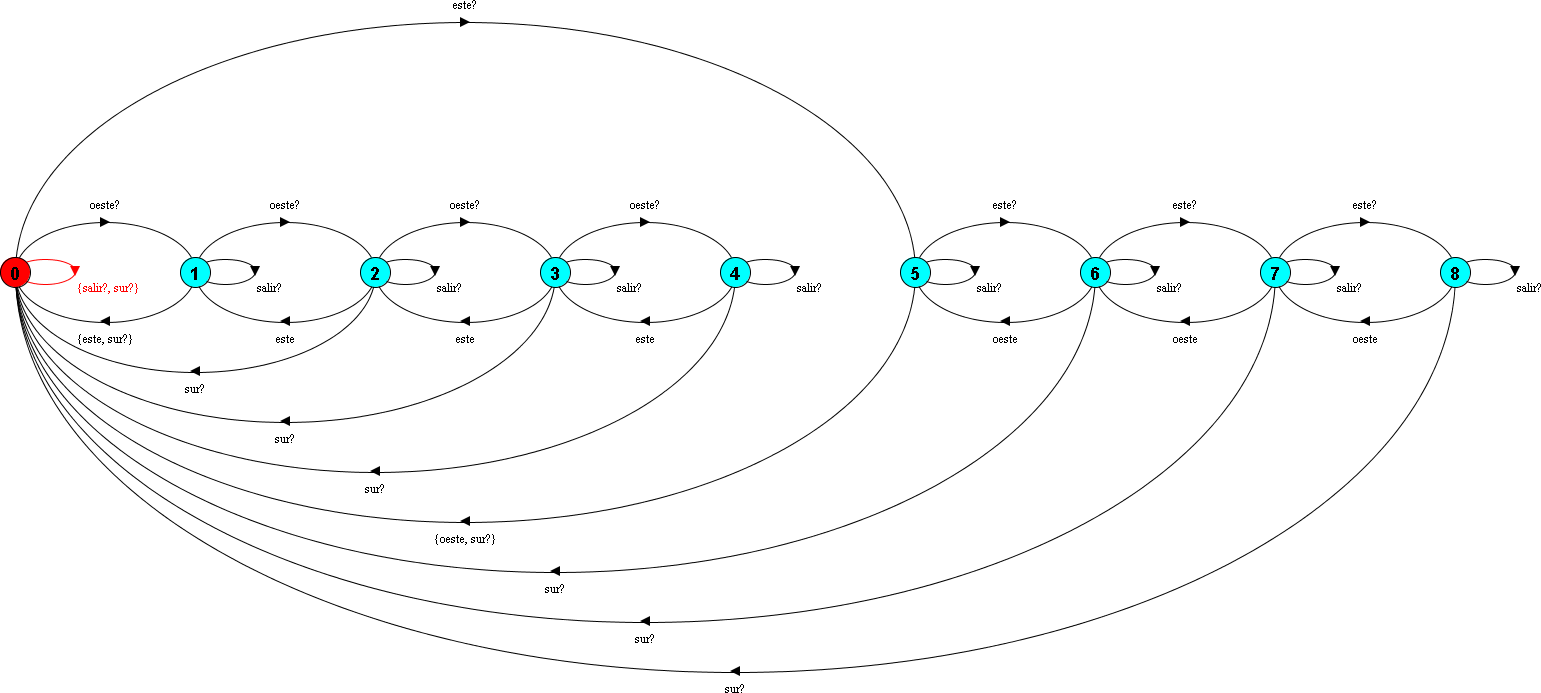
\includegraphics[width=1.0\textwidth]{Imagenes/Laberintos/down_modelo.png}
	\caption{MTS que representa al conocimiento inicial sobre el laberinto que baja.}
	\label{fig:down_modelo}
\end{figure}

El problema está en que no podemos modelar la siguiente condición:
\begin{itemize}
\item
Si podemos movernos una posición horizontalmente, también vamos a poder movernos a \textbf{la misma} posición de la que partimos.
\end{itemize}

Por carecer de esta condición, no podemos saber que las acciones de movimiento horizontal son más seguras que la acción bajar, 
ya que la acción bajar nos puede llevar a un estado perdedor desde un estado ganador, cosa que no puede pasar con las acciones horizontales.

\clearpage

\subsection{Resultado}

\begin{figure}[H]
	\centering
		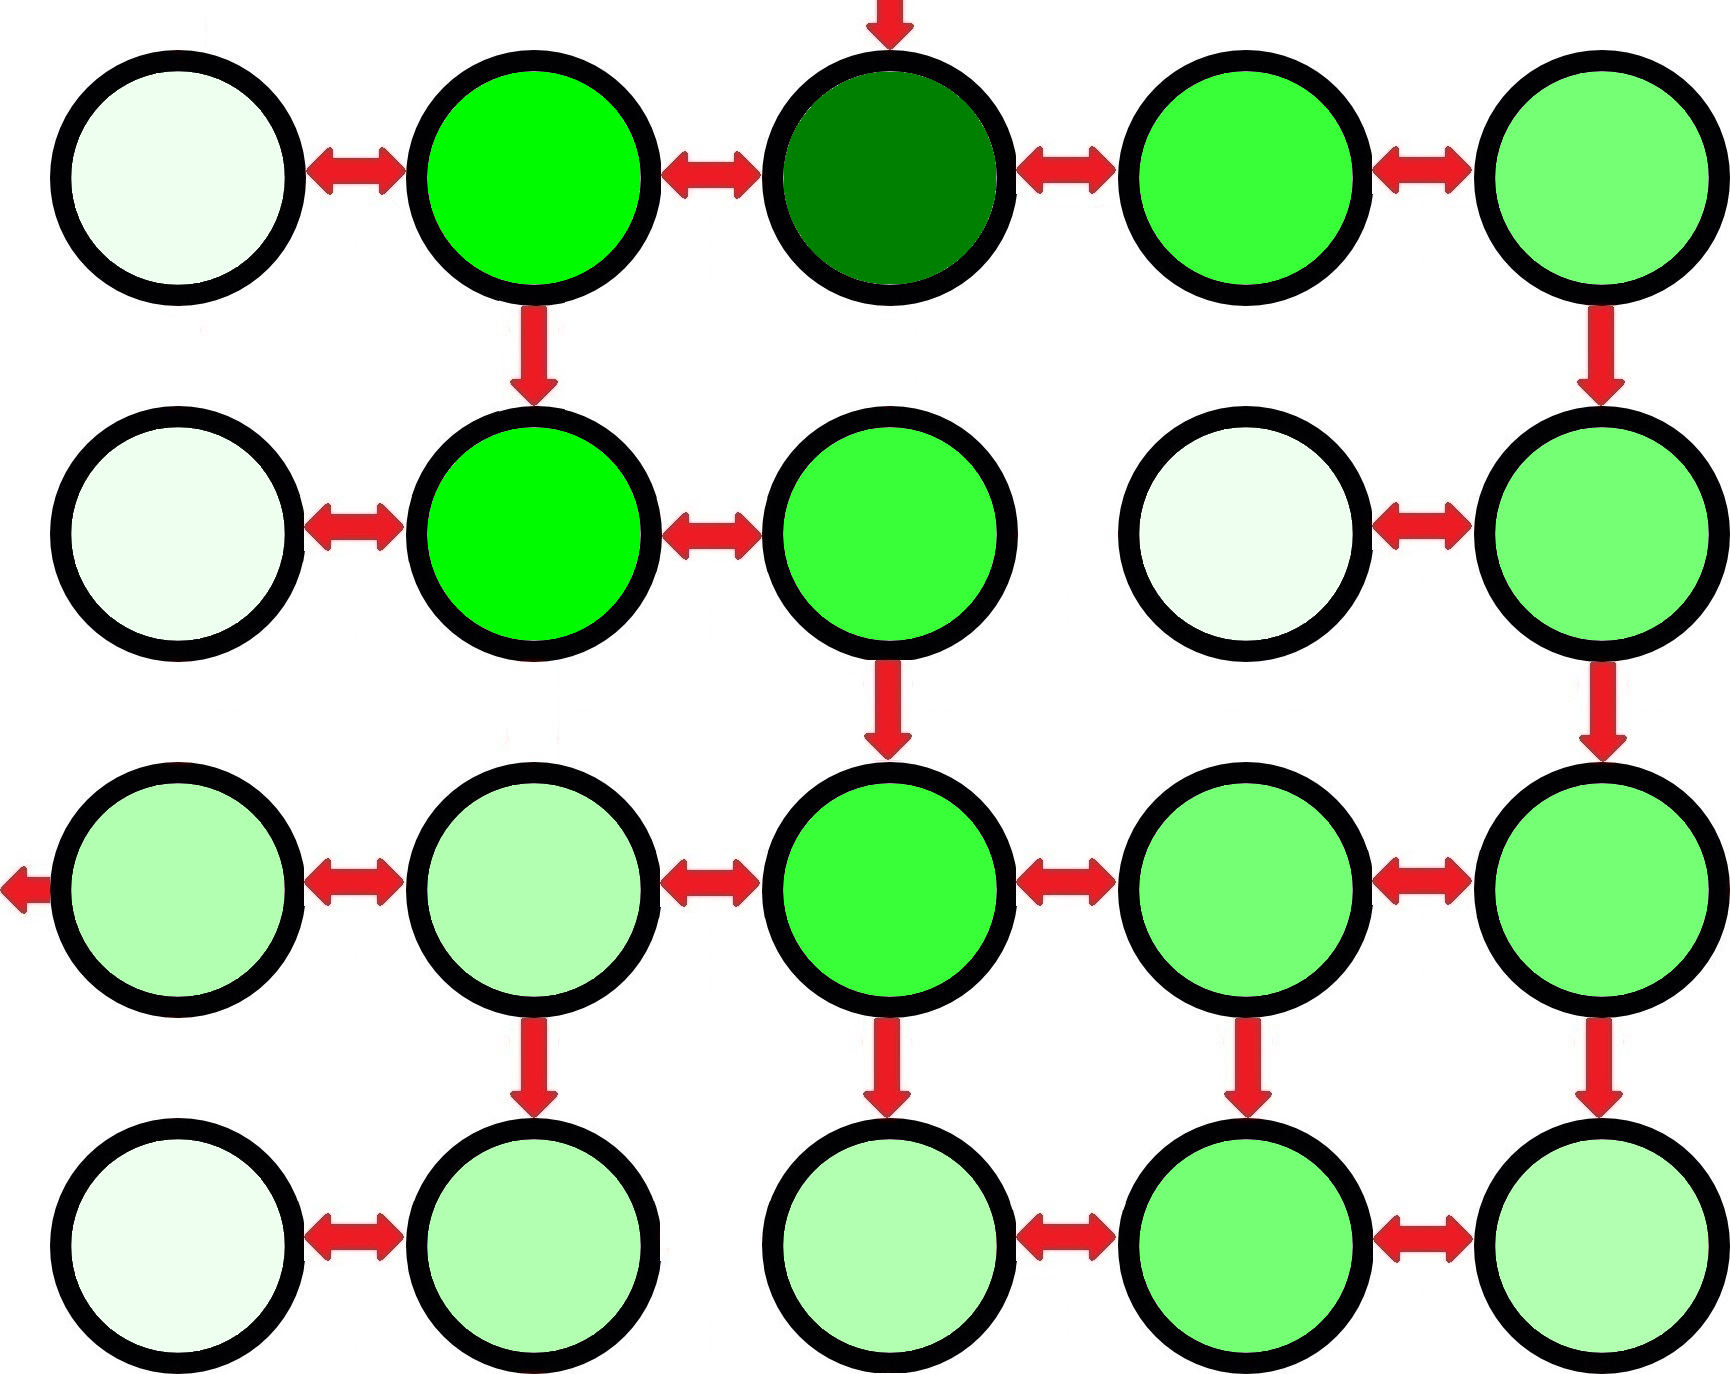
\includegraphics[scale=0.2]{Imagenes/Laberintos/down_calor.png}
	\caption{Mapa de calor del robot en el laberinto que baja.}
	\label{fig:down_calor}
\end{figure}

Utilizando la estrategia Nueva Acción o la estrategia Optimista - Nueva Acción, el robot logra salir del laberinto en 58 pasos, para lo cual fue necesario
realizar un reset en 4 oportunidades. Al no poder distinguir los estados seguros de los que nos pueden llevar a estados perdedores, la estrategia elige arbitrariamente cualquier acción nueva, cayendo varias veces en estados perdedores.

\vspace{\baselineskip}

Utilizando la estrategia Optimista, el robot logra salir del laberinto en 61 pasos, para lo cual fue necesario realizar un reset en 4 oportunidades.

\clearpage

\section{Laberinto con puente}

En este ejemplo, el robot puede moverse libremente entre todas las posiciones contiguas, pero entre las posiciones 7 y 8 hay un puente 
controlado por un agente externo, quien puede cerrar el paso.

\begin{figure}[H]
	\centering
		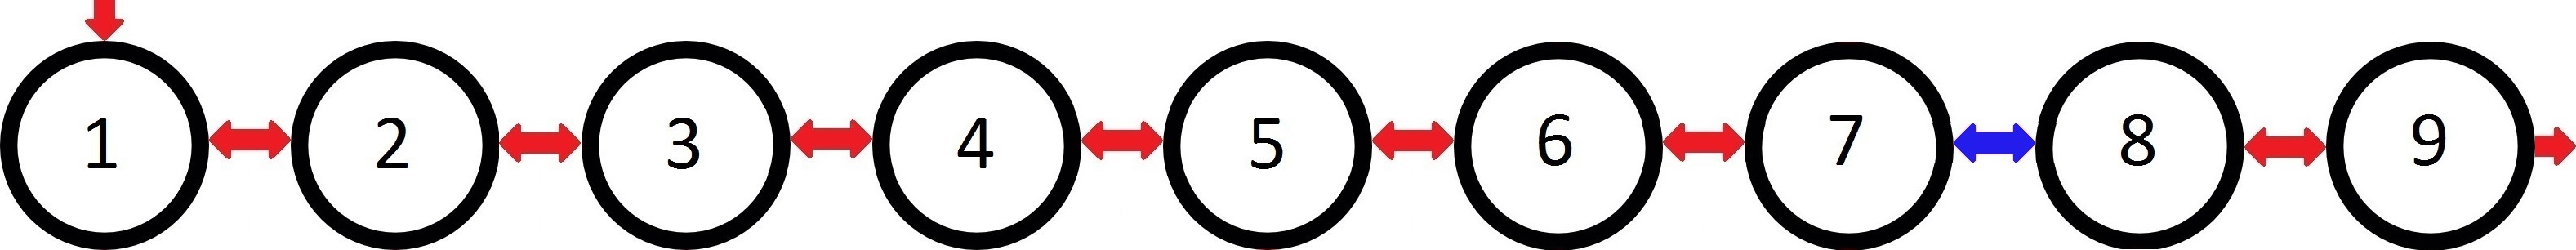
\includegraphics[width=1.0\textwidth]{Imagenes/Laberintos/puente.jpg}
	\caption{Laberinto con puente.}
	\label{fig:puente}
\end{figure}

Este ejemplo introduce un agente externo, por lo cual vamos a necesitar definir:

\begin{itemize}

\item
Un LTS que represente el comportamiento del agente externo. Indica que acciones puede realizar el agente externo en cada momento.

\item
Un MTS que represente nuestro conocimiento inicial sobre el comportamiento del agente externo. 
El robot adquirirá conocimiento sobre el agente externo a medida que pueda observar sus acciones.

\item
Una suposición de dominio sobre el comportamiento del agente externo, la cual garantice que el agente externo no va a impedir 
que alcancemos nuestro objetivo.

\item
Aunque es opcional, vamos a utilizar una lista de acciones que ejecutará el agente externo cíclicamente. 
De esta forma, especificamos su comportamiento para este ejemplo.

En caso de que hubiera más de un agente externo, deberíamos definir estos cuatro items para cada uno de ellos.

\end{itemize}

\clearpage

\subsection{Especificación en MTSA}

\begin{Code}[commandchars=&\[\]]
&fvtextcolor[0000A0][MAPA] = &fvtextcolor[0000A0][M1],
&fvtextcolor[0000A0][M1] = (este   -> &fvtextcolor[0000A0][M2]),
&fvtextcolor[0000A0][M2] = (este   -> &fvtextcolor[0000A0][M3] | oeste  -> &fvtextcolor[0000A0][M1]),
&fvtextcolor[0000A0][M3] = (este   -> &fvtextcolor[0000A0][M4] | oeste  -> &fvtextcolor[0000A0][M2]),
&fvtextcolor[0000A0][M4] = (este   -> &fvtextcolor[0000A0][M5] | oeste  -> &fvtextcolor[0000A0][M3]),
&fvtextcolor[0000A0][M5] = (este   -> &fvtextcolor[0000A0][M6] | oeste  -> &fvtextcolor[0000A0][M4]),
&fvtextcolor[0000A0][M6] = (este   -> &fvtextcolor[0000A0][M7] | oeste  -> &fvtextcolor[0000A0][M5]),
&fvtextcolor[0000A0][M7] = (cruzar -> &fvtextcolor[0000A0][M8] | oeste  -> &fvtextcolor[0000A0][M6]),
&fvtextcolor[0000A0][M8] = (este   -> &fvtextcolor[0000A0][M9] | cruzar -> &fvtextcolor[0000A0][M7]),
&fvtextcolor[0000A0][M9] = (oeste  -> &fvtextcolor[0000A0][M8] | ganar  -> &fvtextcolor[0000A0][M9]).

&fvtextcolor[0000A0][PUENTE] = &fvtextcolor[0000A0][PUENTE_CERRADO],
&fvtextcolor[0000A0][PUENTE_CERRADO] = (abrir  -> &fvtextcolor[0000A0][PUENTE_ABIERTO] | cerrar -> &fvtextcolor[0000A0][PUENTE_CERRADO]),
&fvtextcolor[0000A0][PUENTE_ABIERTO] = (abrir  -> &fvtextcolor[0000A0][PUENTE_ABIERTO] | cruzar -> &fvtextcolor[0000A0][PUENTE_ABIERTO] | 
                  cerrar -> &fvtextcolor[0000A0][PUENTE_CERRADO]).

&fvtextcolor[0000A0][MTS_MAPA]   = (este?   -> &fvtextcolor[0000A0][MTS_MAPA]   | oeste?  -> &fvtextcolor[0000A0][MTS_MAPA]   | 
              cruzar? -> &fvtextcolor[0000A0][MTS_MAPA]   | ganar?  -> &fvtextcolor[0000A0][MTS_MAPA]).
							
&fvtextcolor[0000A0][MTS_PUENTE] = (abrir?  -> &fvtextcolor[0000A0][MTS_PUENTE] | cerrar? -> &fvtextcolor[0000A0][MTS_PUENTE] | 
              cruzar? -> &fvtextcolor[0000A0][MTS_PUENTE]).

&fvtextcolor[0000FF][set] &fvtextcolor[0000A0][Controllable_puente] = {este, oeste, cruzar, ganar}

&fvtextcolor[0000FF][fluent] &fvtextcolor[0000A0][F_Ganar] = <ganar, &fvtextcolor[0000A0][Controllable_puente]\{ganar}>
&fvtextcolor[0000FF][assert] &fvtextcolor[0000A0][A_Ganar] = &fvtextcolor[0000A0][F_Ganar]

&fvtextcolor[0000FF][fluent] &fvtextcolor[0000A0][F_PuedeCruzar] = <abrir, cruzar>
&fvtextcolor[0000FF][assert] &fvtextcolor[0000A0][PuedeCruzar]   = &fvtextcolor[0000A0][F_PuedeCruzar]

&fvtextcolor[0000FF][controllerSpec] &fvtextcolor[0000A0][GOAL_PUENTE] = {
    assumption   = {&fvtextcolor[0000A0][PuedeCruzar]}
    liveness     = {&fvtextcolor[0000A0][A_Ganar]}
    controllable = {&fvtextcolor[0000A0][Controllable_puente]}
}

&fvtextcolor[0000FF][exploration] &fvtextcolor[0000A0][PUENTE_CON_SALIDA] = {
    environment         = {&fvtextcolor[0000A0][MAPA], &fvtextcolor[0000A0][PUENTE]},
    model               = {&fvtextcolor[0000A0][MTS_MAPA], &fvtextcolor[0000A0][MTS_PUENTE]},
    goal                = {&fvtextcolor[0000A0][GOAL_PUENTE]},
    environment_actions = {{cerrar, cerrar, cerrar, cerrar, cerrar,
                            cerrar, cerrar, cerrar, cerrar, cerrar, 
                            abrir, abrir, abrir}}
}
\end{Code}

\clearpage

\subsection{Estrategias}

Este ejemplo cuenta con un agente externo. La estrategia Optimista no está preparada para estos casos, por lo cual entra en un ciclo que le impide adquirir
nuevo conocimiento. Al utilizar las estrategias Nueva Acción u Optimista - Nueva Acción, el resultado es el mismo.

\subsection{Análisis de los modelos}

Como el robot observa todas las acciones del agente externo, al final de la exploración, el MTS que representa su comportamiento está completamente refinado.

\begin{figure}[H]
	\centering
		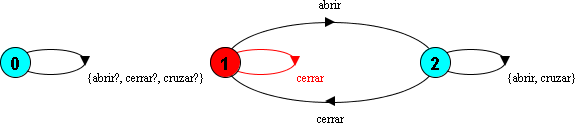
\includegraphics[width=1.0\textwidth]{Imagenes/Laberintos/puente_modelo_puente.png}
	\caption{MTS que representa al conocimiento adquirido sobre el agente externo del laberinto con puente.}
	\label{fig:puente_modelo_puente}
\end{figure}

En cuanto al mapa, la única acción no ejecutada es cruzar desde el estado 8 al estado 7.

\begin{figure}[H]
	\centering
		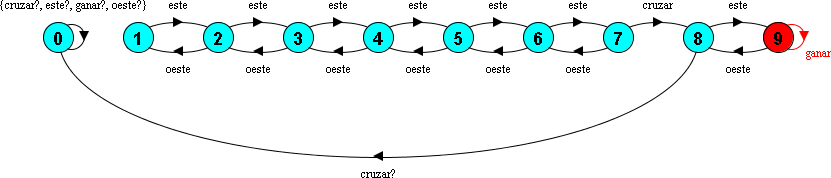
\includegraphics[width=1.0\textwidth]{Imagenes/Laberintos/puente_modelo_mapa.png}
	\caption{MTS que representa al conocimiento adquirido sobre el laberinto con puente.}
	\label{fig:puente_modelo_mapa}
\end{figure}

\subsection{Análisis de la traza}

El robot logra salir del laberinto en 30 pasos. En el siguiente video \url{https://youtu.be/wec0GPml9dc} podemos observar, movimiento a movimiento,
como cambian los modelos de conocimiento que el robot tiene sobre el entorno, el cual en este caso es el camino que tiene un puente, y sobre el agente
externo, que en este caso, es quien decide cuando el puente se abre o se cierra. El video nos permite ver de una forma más clara como las acciones
nunca antes realizadas aportan información, y como el robot necesita volver a posiciones no completamente exploradas para incrementar su conocimiento.

\vspace{\baselineskip}
Podemos observar que cuando el robot termina de explorar completamente los estados 1 a 7, 
va hasta el estado 7 a esperar que el agente externo abra el puente, en vez de esperarlo en su estado actual, ya que solamente desde el estado 7 
puede beneficiarse de las acciones del agente externo.

\vspace{\baselineskip}

El robot sabe que el agente externo va a abrir el puente por la suposición de dominio que tenemos. En caso de no tener esta suposición, 
en vez de esperar, el robot asumiría que no se puede garantizar el cumplimiento del objetivo, ya que el agente externo podría no abrir el puente nunca.

\begin{figure}[H]
	\centering
		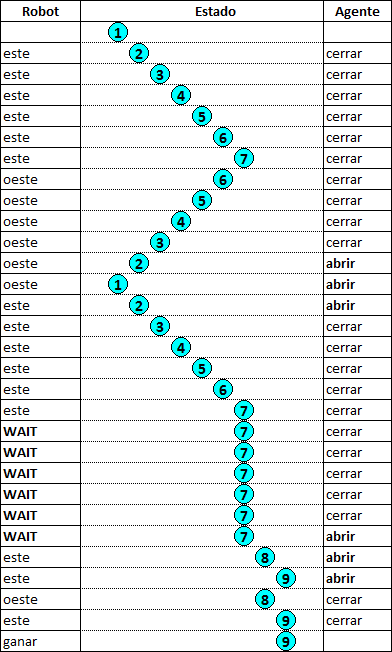
\includegraphics[width=0.7\textwidth]{Imagenes/Laberintos/puente_traza.png}
	\caption{Traza del robot en el laberinto con puente.}
	\label{fig:puente_traza}
\end{figure}

\chapter{Conclusiones}

En el final de esta tesis, hay cuatro temas interesantes para analizar.

\vspace{\baselineskip}
El primer tema a analizar es la integración de la exploración a la herramienta MTSA, la cual se puede ver en detalle en el 
siguiente capítulo. 
Se extendió el lenguaje de Procesos de Estados Finitos (FSP) para que sea sencillo definir exploraciones, se agregaron botones 
para dar control total sobre la exploración y se agregó una nueva forma de visualización de los modelos, más flexible, mediante 
la pestaña Layout.

\vspace{\baselineskip}
La herramienta nos permite visualizar la exploración paso a paso, tanto la traza de la exploración como la 
evolución de los modelos. También nos permite avanzar inmediatamente la cantidad de pasos necesarios, para luego ver en detalle 
una etapa más avanzada de la exploración. Es posible explorar siguiendo la estrategia de exploración, e intervenir manualmente 
en las decisiones en caso de ser necesario.

\vspace{\baselineskip}
El segundo tema importante es el algoritmo de exploración. Resuelve el problema correctamente en caso de contar con una estrategia 
adecuada, y tiene la flexibilidad suficiente como para permitir las ventajas mencionadas en el párrafo anterior. Su mayor 
inconveniente es la complejidad temporal.

\vspace{\baselineskip}
Por cada iteración del algoritmo es necesario realizar una síntesis de controladores para decidir si es necesario seguir explorando 
(dos síntesis en el caso de que sea necesario un reset), una síntesis para la estrategia Síntesis, y un número variable de síntesis 
para la estrategia Nueva Acción en caso de que no haya acciones nuevas en el estado actual.

\vspace{\baselineskip}
La síntesis de controladores es un proceso computacionalmente caro. Cada modelo que sintetizamos es muy similar al modelo sintetizado 
en la iteración anterior, sería interesante como trabajo a futuro poder utilizar la síntesis anterior para realizar la próxima en 
vez de volver a realizar el proceso desde el comienzo. Esto afectaría considerablemente el rendimiento del algoritmo en forma favorable.

\vspace{\baselineskip}
El tercer tema interesante surge del ejemplo del laberinto que baja. En los MTSs, al utilizar una transición posible, perdemos la forma 
de especificar que podemos volver exactamente al mismo estado del cual sale la transición posible. Sería de bastante utilidad, como 
trabajo a futuro, extender los MTSs de alguna forma que permita especificar estos detalles.

\begin{figure}[H]
	\centering
		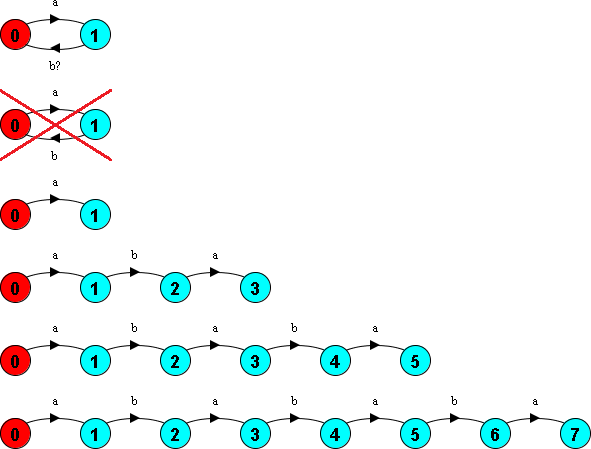
\includegraphics[width=1.0\textwidth]{Imagenes/Otros/Limitaciones.png}
	\caption{Limitaciones del modelado con MTSs}
	\label{fig:Limitaciones}
\end{figure}

Como se puede ver en la imagen, el MTS no se puede refinar al primero de los LTSs, sino que los LTSs que pueden ser refinados a partir 
del MTS son de la forma del segundo LTS en adelante.

\vspace{\baselineskip}
Por último, el cuarto tema fundamental a tener en cuenta es la estrategia presentada. La estrategia resuelve el problema de salir de 
un laberinto, incluso con la participación de agentes externos que influyen sobre el entorno. Pero lo único que busca la estrategia 
es determinar si es posible o no cumplir el objetivo propuesto, como trabajo a futuro se puede mejorar en varios aspectos para reducir 
la cantidad de pasos necesarios para hallar una respuesta.

\vspace{\baselineskip}
Por ejemplo, en caso de tener varias acciones disponibles, siempre las va a elegir basándose en el mismo orden arbitrario. En consecuencia, 
la exploración siempre de preferencia a una dirección por sobre las demás, lo cual puede ser perjudicial. Sería interesante definir 
la forma en la que se elige una acción en caso de que haya varias acciones que cumplen los requisitos de la estrategia, ya sea de forma 
aleatoria o mediante una heurística.

\vspace{\baselineskip}
Algo similar ocurre cuando la estrategia necesita dirigirse hacia otro estado, por encontrarse en un estado completamente explorado. 
En la versión actual de la estrategia se intenta llegar a un estado elegido de forma arbitraria entre los que no fueron completamente 
explorados. Hay varias opciones que podrían llegar a ser más adecuadas, como por ejemplo dirigirse hacia el estado más cercano a la 
posición actual, al más cercano al inicio para hacer una exploración de estilo BFS (Breadth First Search), o al más lejano para explorar 
en forma DFS (Depth First Search) o intentar heurísticas más complicadas, quizás utilizando la información sobre el entorno de la cual 
disponemos en el momento.

\vspace{\baselineskip}
Además de las posibles optimizaciones sobre la estrategia presentada, sería interesante elaborar estrategias nuevas para resolver el 
problema, o estrategias adecuadas para circunstancias particulares, como no disponer de un modelo del entorno, o no poder distinguir 
inequívocamente las posiciones en el entorno.

\vspace{\baselineskip}
En conclusión, este trabajo es un primer paso, el cual brinda las herramientas necesarias para comenzar a investigar el campo de la 
exploración mediante MTSs. Todavía queda mucho por hacer en varios aspectos diferentes, ya que es un tema nuevo, extenso e interesante.
\chapter{Apéndice}

\subsubsection{Manual de usuario}

Se explica detalladamente cómo utilizar la herramienta MTSA para la exploración. 
Mostramos cómo deben ser los inputs, cuales son las funcionalidades de la herramienta, como nos permite visualizar 
la exploración y avanzar en ella, y cuales son los output que nos brinda.

\subsubsection{Ejemplo de exploración en MTSA}

Mostramos con un ejemplo el seguimiento de una exploración en la herramienta MTSA. 
Comenzamos con un modelo, el cual incluye un agente externo, y mostramos las particularidades de la exploración hasta obtener un resultado. 
Vemos como van evolucionando los modelos, particularidades de la estrategia elegida y cómo visualizamos el paso a paso de la exploración.



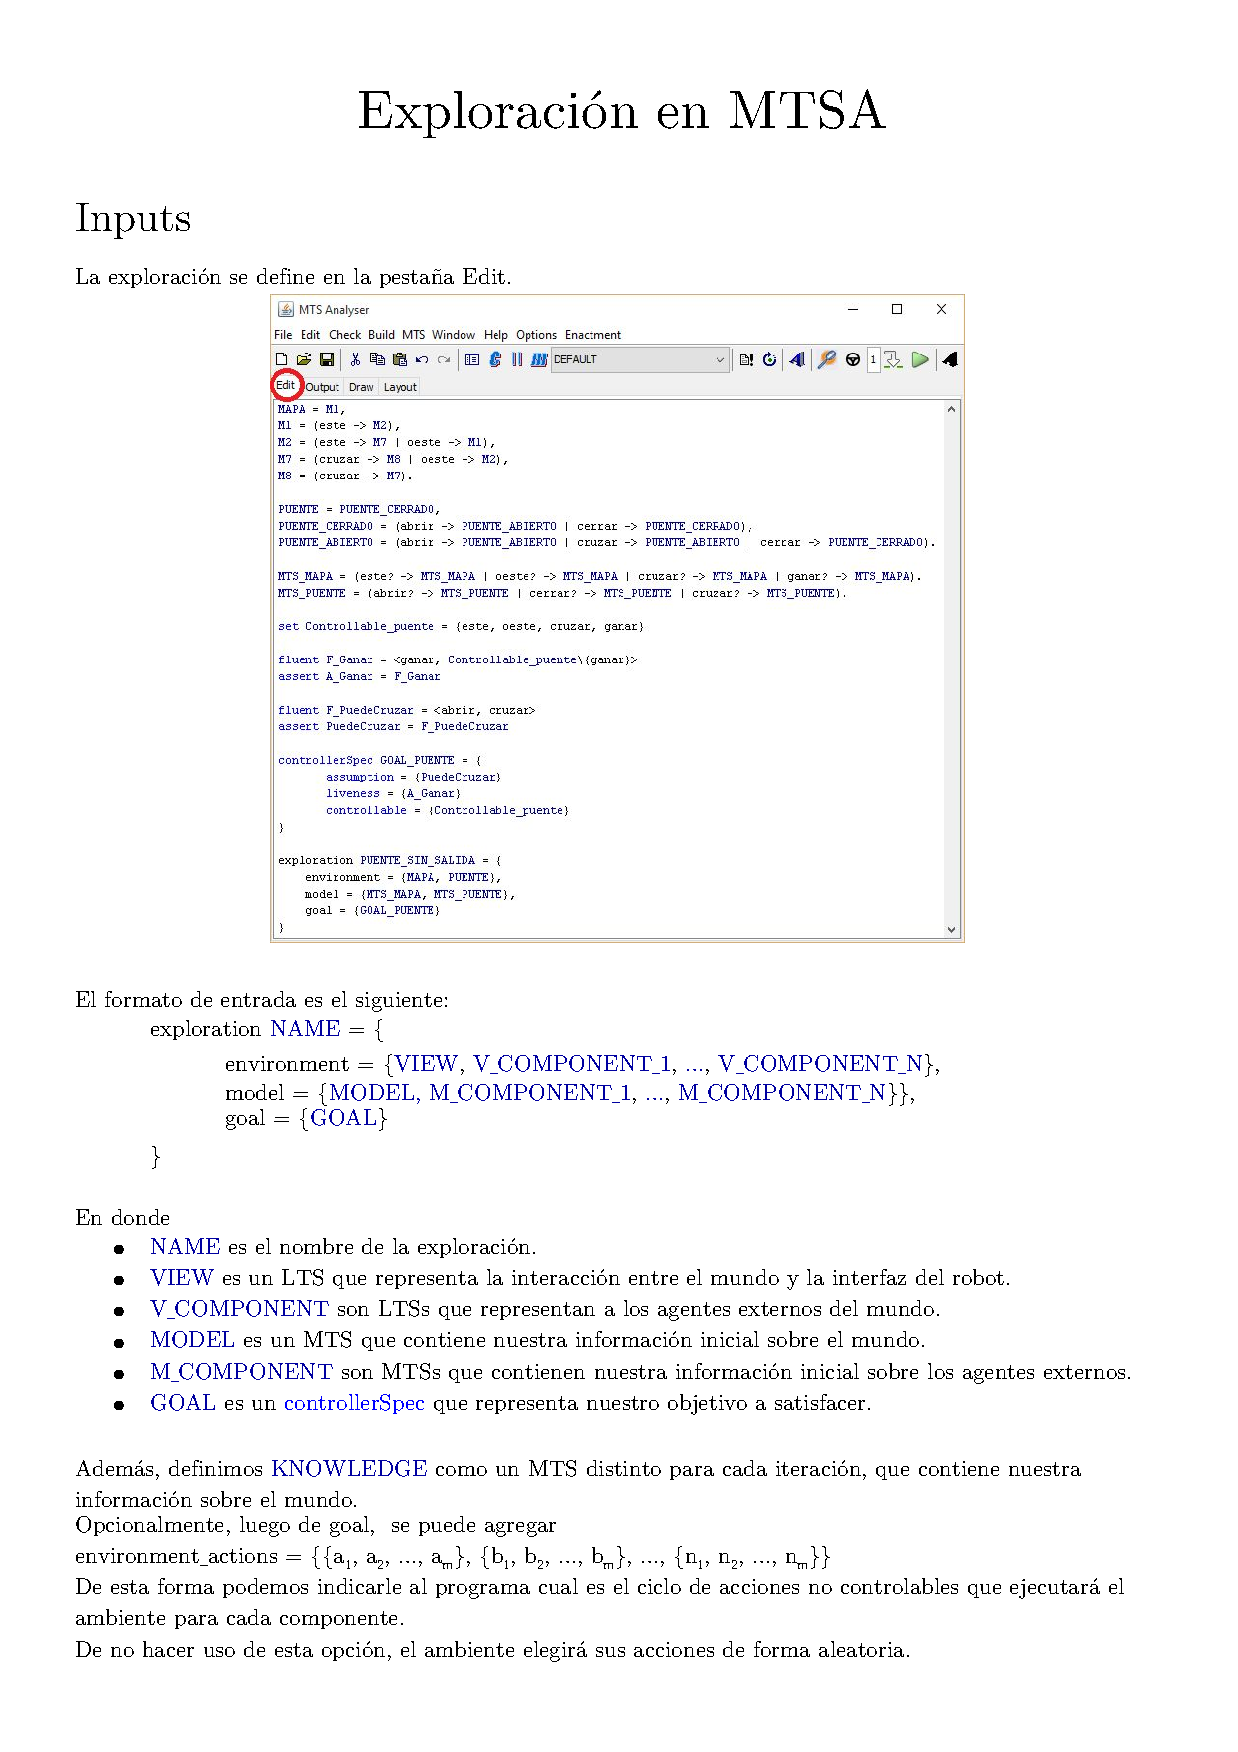
\includepdf[pages = -]{Manual.pdf}
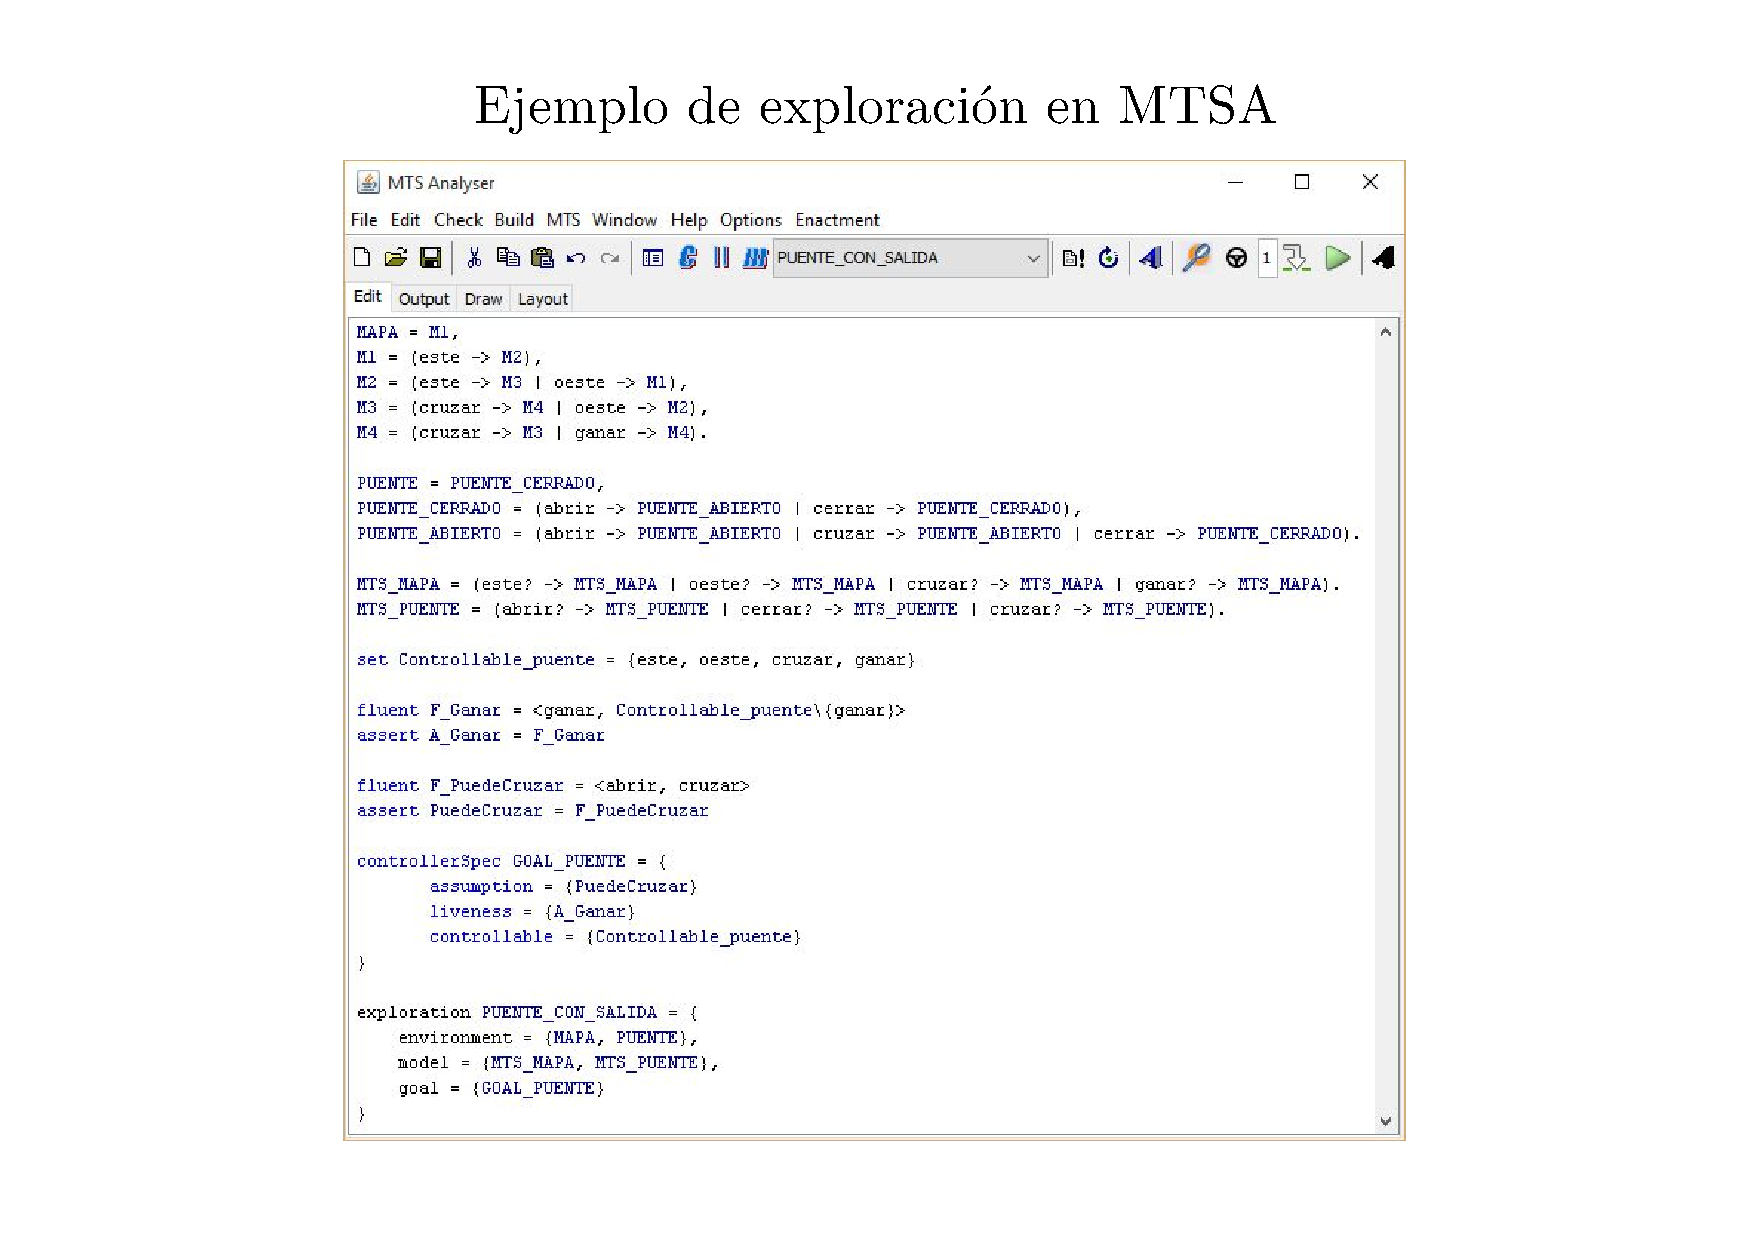
\includepdf[pages = -]{Ejemplo.pdf}

%%%% BIBLIOGRAFIA
\backmatter
\bibliographystyle{plain}
\bibliography{bibliografia}

\end{document}